% Hak cipta 2025 oleh Robert Hildebrand
%Karya ini dilisensikan berdasarkan
%Lisensi Internasional Creative Commons Atribusi-BerbagiSerupa 4.0 (CC BY-SA 4.0)
%Lihat http://creativecommons.org/licenses/by-sa/4.0/
\chapter{Metode Simpleks}
\label{ch:simplex-dictionary}
\begin{outcome}
\begin{itemize}
\item Mengonversi program linier ke bentuk standar
\item Merumuskan ulang program linier dari sudut pandang basis yang berbeda
\item Mendefinisikan \emph{solusi basis} dan \emph{solusi basis layak}
\item Menjelaskan kondisi optimalitas dari sudut pandang suatu perumusan ulang
\item Mengembangkan \emph{Metode Simpleks} yang melakukan \emph{pivot} melalui solusi-solusi basis layak
\end{itemize}
\end{outcome}

\begin{quote}
\itshape Bayangkan Anda mendaki menuju titik tertinggi sebuah lapangan berpagar pada malam tanpa bulan. Senter Anda hanya menerangi tanah di kaki Anda: sudut tempat Anda berdiri dan garis-garis pagar yang menjauh darinya. Sebuah strategi yang masuk akal pun muncul: arahkan cahaya sepanjang setiap garis pagar; jika salah satunya menanjak, ikuti hingga sudut berikutnya lalu periksa lagi; jika tidak ada yang menanjak, berhentilah. Fakta luar biasa dalam bab ini adalah bahwa untuk program linier, strategi berpandangan dekat ini dijamin berakhir di titik tertinggi seluruh lapangan. Aljabar dari ``mengarahkan senter'' merupakan suatu perumusan ulang program linier yang disebut \emph{kamus}.
\end{quote}

Pada bagian ini, kita akan mengembangkan \emph{Metode Simpleks}. Algoritma ini telah dipuji sebagai salah satu algoritma terpenting abad ke-20. Algoritma ini secara iteratif akan menemukan solusi titik sudut yang lebih baik bagi suatu program linier sampai dapat membuktikan optimalitas.

Untuk mengimplementasikan algoritma simpleks, pertama-tama kita harus membahas suatu \emph{Bentuk Standar} untuk merepresentasikan program linier. Setelah itu, kita akan membahas struktur program linier dalam bentuk ini menggunakan notasi matriks dan menunjukkan bagaimana suatu program linier dapat ditransformasikan ke representasi baru. Representasi baru ini akan menjadi tulang punggung algoritma simpleks. Kita akan melakukan \emph{pivot} antar-titik sudut, dan setiap titik sudut akan memiliki representasi baru program linier yang membantu kita memahami cara memilih titik sudut baru yang akan dituju.

Secara keseluruhan, algoritma ini berjalan sangat cepat dalam praktik. Di sini, kita akan mempelajari versi dasar algoritma tersebut, tetapi perhatikan bahwa pemecah mutakhir menggunakan sejumlah kiat untuk membuat proses ini sangat cepat. Program linier dengan jutaan variabel dapat diselesaikan!

\section{Bentuk Standar}
\label{sec:standard-form}

Untuk menyelesaikan program linier menggunakan metode seperti algoritma simpleks, masalahnya terlebih dahulu harus dikonversi ke bentuk standar. Hal ini memastikan bahwa masalah mengikuti struktur yang seragam sehingga lebih mudah dianalisis dan diselesaikan secara algoritmik.

Suatu program linier berada dalam \emph{bentuk standar} jika memenuhi semua hal berikut:
\begin{itemize}
    \item Fungsi objektifnya berupa maksimisasi.
    \item Semua kendala berupa persamaan (yaitu, berbentuk \( = \)).
    \item Semua variabel dibatasi dari bawah oleh nol (yaitu, \( x_i \geq 0 \)).
\end{itemize}

\begin{definition}{Bentuk Standar}\label{def:standardform}
Suatu program linier berada dalam \emph{bentuk standar} jika ditulis sebagai
\begin{align*}
\max \ \ &\c^\top \x \\
s.t. \ \ & A\x = \b\\
& \x \geq 0.
\end{align*}
\end{definition}

\subsection{Mengonversi ke Bentuk Standar}
Sekarang kita menjelaskan cara menangani setiap aspek ini langkah demi langkah, termasuk subkasus dan contoh yang umum.

\subsubsection*{1. Fungsi Objektif: Mengonversi Minimisasi ke Maksimisasi}

Jika program linier diberikan sebagai masalah minimisasi, kita mengonversinya menjadi masalah maksimisasi dengan mengalikan fungsi objektif dengan \( -1 \). Transformasi ini tidak memengaruhi daerah layak, dan pemaksimum fungsi baru akan menjadi peminimum fungsi semula.

\begin{example}{Mengonversi Min ke Maks}
Perhatikan fungsi objektif berikut:
\[
\min \; 3x_1 + 4x_2.
\]
Untuk mengonversinya menjadi maksimisasi, kita mengalikan seluruh ekspresi dengan \( -1 \):
\[
\max \; (-3x_1 - 4x_2).
\]
Sekarang masalah tersebut dapat ditangani menggunakan metode standar yang mengasumsikan fungsi objektif berupa maksimisasi.
\end{example}
\newpage
\subsubsection*{2. Kendala: Mengonversi Pertidaksamaan Menjadi Persamaan}

Semua kendala pertidaksamaan harus ditransformasikan menjadi persamaan menggunakan variabel slack atau surplus, yang merepresentasikan selisih antara ruas kiri dan ruas kanan kendala.

\begin{itemize}
    \item[(a)] \textbf{Mengonversi \( \leq \) menjadi \( = \) menggunakan variabel slack.}

    Variabel slack ditambahkan untuk ``mengisi kesenjangan'' pada kendala \( \leq \) dan harus nonnegatif.

    \begin{example}{Variabel Slack untuk \(\leq\)}
    Misalkan kita memiliki kendala:
    \[
    x_1 + 2x_2 \leq 5.
    \]
    Kita memperkenalkan variabel baru \( s_1 \geq 0 \), yang disebut variabel slack, dan menulis ulang kendala sebagai:
    \[
    x_1 + 2x_2 + s_1 = 5.
    \]
    Di sini, \( s_1 \) merepresentasikan bagian ruas kanan yang tidak digunakan (yaitu, seberapa jauh ruas kiri dari 5).
    \end{example}

    \item[(b)] \textbf{Mengonversi \( \geq \) menjadi \( = \) menggunakan variabel surplus.}

    Variabel surplus dikurangkan dari ruas kiri kendala \( \geq \) untuk mengonversinya menjadi persamaan. Variabel ini juga harus nonnegatif.

    \begin{example}{Variabel Surplus untuk \(\geq\)}
    Perhatikan kendala:
    \[
    x_1 - x_2 \geq 3.
    \]
    Kita memperkenalkan variabel baru \( s_2 \geq 0 \), yang disebut variabel surplus, dan menulis ulang kendala sebagai:
    \[
    x_1 - x_2 - s_2 = 3.
    \]
    Dalam kasus ini, \( s_2 \) menyatakan besarnya kelebihan ruas kiri atas 3.
    \end{example}
\end{itemize}

\subsubsection*{3. Batas Variabel: Memastikan Semua Variabel Nonnegatif}

Bentuk standar mengharuskan semua variabel memenuhi \( x_i \geq 0 \). Jika ada variabel yang tidak dibatasi dari bawah atau dibatasi dengan cara lain, kita melakukan substitusi variabel untuk memberlakukan kondisi ini.

\begin{itemize}
    \item[(a)] \textbf{Mengonversi \( x_i \leq 0 \) menjadi \( x_i' \geq 0 \) dengan mengganti nama dan menegasikannya.}

    Jika suatu variabel dibatasi agar nonpositif, kita dapat mendefinisikan variabel nonnegatif baru sebagai negatif dari variabel tersebut.

    \begin{example}{Mengganti Nama dan Menegasikan untuk \(\leq 0\)}
    Misalkan \( x_3 \leq 0 \). Definisikan \( x_3' = -x_3 \), yang mengimplikasikan \( x_3' \geq 0 \). Kemudian substitusikan:
    \[
    x_3 = -x_3', \quad \text{dengan } x_3' \geq 0.
    \]
    Transformasi ini memungkinkan kita memberlakukan nonnegativitas dalam bentuk standar.
    \end{example}

    \item[(b)] \textbf{Mengonversi variabel bebas menjadi selisih dua variabel nonnegatif.}

    Jika suatu variabel bebas dalam tanda (yaitu, dapat bernilai positif atau negatif), kita menyatakannya sebagai selisih dua variabel nonnegatif baru.

    \begin{example}{Variabel Bebas Menjadi Dua Variabel}
    Misalkan \( x_4 \) bebas. Kita mendefinisikan:
    \[
x_4 = x_4^+ - x_4^-, \quad \text{dengan } x_4^+, x_4^- \geq 0.
    \]
    Di sini, \( x_4^+ \) menangkap bagian positif dan \( x_4^- \) menangkap bagian negatif. Paling banyak salah satunya akan bernilai taknol dalam suatu solusi basis layak.
    \end{example}
\end{itemize}

\medskip

Setelah melakukan transformasi-transformasi ini, program linier yang dihasilkan akan berada dalam bentuk standar dan siap diselesaikan melalui metode simpleks atau teknik standar lainnya.

\begin{example}{Konversi Lengkap ke Bentuk Standar}
Perhatikan program linier berikut:

\[
\begin{aligned}
\min \quad & 2x_1 - 3x_2 + x_3 \\
\st \quad 
& x_1 - x_2 \leq 4, \\
& 2x_1 + x_3 = 7, \\
& x_2 - x_3 \geq 2, \\
& x_1 \text{ bebas tanda}, \quad x_2 \geq 0, \quad x_3 \text{ bebas tanda}.
\end{aligned}
\]

Sekarang kita akan mengonversi masalah ini ke bentuk standar.

\medskip
\textbf{Langkah 1: Mengonversi fungsi objektif menjadi maksimisasi.}

Karena masalahnya berupa minimisasi, kita mengalikan fungsi objektif dengan \( -1 \):
\[
\max \; (-2x_1 + 3x_2 - x_3).
\]

\medskip
\textbf{Langkah 2: Mengganti variabel bebas.}

Baik \( x_1 \) maupun \( x_3 \) adalah variabel bebas. Kita menyatakannya sebagai selisih dua variabel nonnegatif:
\[
x_1 = x_1^+ - x_1^-, \quad x_3 = x_3^+ - x_3^-, \quad \text{dengan } x_1^+, x_1^-, x_3^+, x_3^- \geq 0.
\]

Substitusikan variabel-variabel ini ke dalam fungsi objektif dan kendala.

\smallskip
\textbf{Fungsi objektif baru:}
\[
\max \; [-2(x_1^+ - x_1^-) + 3x_2 - (x_3^+ - x_3^-)] = \max \; (-2x_1^+ + 2x_1^- + 3x_2 - x_3^+ + x_3^-).
\]

\smallskip
\textbf{Kendala baru:}
\begin{align*}
(x_1^+ - x_1^-) - x_2 &\leq 4 \quad &\text{(kendala semula ke-1)} \\
2(x_1^+ - x_1^-) + (x_3^+ - x_3^-) &= 7 \quad &\text{(kendala semula ke-2)} \\
x_2 - (x_3^+ - x_3^-) &\geq 2 \quad &\text{(kendala semula ke-3)}
\end{align*}

\medskip
\textbf{Langkah 3: Mengonversi pertidaksamaan menjadi persamaan.}

\begin{itemize}
    \item Tambahkan variabel slack \( s_1 \geq 0 \) ke kendala pertama:
    \[
    x_1^+ - x_1^- - x_2 + s_1 = 4
    \]

    \item Kendala kedua sudah berupa persamaan:
    \[
    2x_1^+ - 2x_1^- + x_3^+ - x_3^- = 7
    \]

    \item Kurangkan variabel surplus \( s_2 \geq 0 \) dari kendala ketiga:
    \[
    x_2 - x_3^+ + x_3^- - s_2 = 2
    \]
\end{itemize}

\medskip
\textbf{Bentuk standar akhir:}

\[
\begin{aligned}
\max \quad & -2x_1^+ + 2x_1^- + 3x_2 - x_3^+ + x_3^- \\
\st \quad 
& x_1^+ - x_1^- - x_2 + s_1 = 4 \\
& 2x_1^+ - 2x_1^- + x_3^+ - x_3^- = 7 \\
& x_2 - x_3^+ + x_3^- - s_2 = 2 \\
& x_1^+, x_1^-, x_2, x_3^+, x_3^-, s_1, s_2 \geq 0.
\end{aligned}
\]

Sekarang masalah ini berada dalam bentuk standar: masalah maksimisasi dengan kendala persamaan dan semua variabel nonnegatif.
\end{example}

\begin{remark}{Transformasi Variabel Mempertahankan Makna Solusi}{}
Untuk mengonversi suatu program linier ke bentuk standar, kita sering memperkenalkan variabel baru:
\begin{itemize}
    \item Variabel slack untuk mengonversi kendala \( \leq \) menjadi persamaan,
    \item Variabel surplus untuk kendala \( \geq \),
    \item Memecah variabel bebas sebagai \( x_j = x_j^+ - x_j^- \),
    \item Menegasikan variabel dengan \( x_j \leq 0 \).
\end{itemize}

Transformasi ini dapat mengubah jumlah variabel dan cara solusi dinyatakan, tetapi:
\begin{enumerate}
    \item Setiap solusi layak bagi masalah hasil transformasi berkorespondensi dengan suatu solusi layak bagi masalah semula.
    \item Setiap solusi optimal dari masalah hasil transformasi menghasilkan solusi optimal bagi masalah semula.
\end{enumerate}

Jadi, meskipun \emph{bentuk} solusi mungkin tampak berbeda, \emph{makna} dan \emph{nilai} solusi tetap dipertahankan.
\end{remark}

\begin{figure}[h]
\centering
\begin{tikzpicture}[node distance=1.5cm and 4.5cm, every node/.style={font=\small}]
\tikzstyle{box} = [draw, fill=blue!10, rounded corners, text width=4.5cm, minimum height=1.3cm, align=center]
\tikzstyle{arrow} = [-{Stealth}, thick]

% Nodes
\node[box] (original) {PL semula\\ (min atau maks, variabel bebas tanda, pertidaksamaan)};
\node[box, right=of original] (transformed) {PL hasil transformasi dalam bentuk kanonik\\ (maks, semua persamaan, variabel $\geq 0$)};
\node[box, below=of original] (origsol) {Solusi PL semula};
\node[box, below=of transformed] (transsol) {Solusi PL hasil transformasi};

% Arrows
\draw[arrow] (original) -- (transformed) node[midway, above] {\footnotesize transformasi variabel};
\draw[arrow] (transformed) -- (original) node[midway, below] {\footnotesize tafsirkan di ruang semula};

\draw[arrow] (transsol) -- (origsol) node[midway, below] {\footnotesize petakan kembali (mis., $x_j = x_j^+ - x_j^-$)};
\draw[arrow] (origsol) -- (transsol) node[midway, above] {\footnotesize enkode ke bentuk kanonik};

\end{tikzpicture}
\caption{Korespondensi antara solusi bentuk semula dan bentuk kanonik.}
\end{figure}

\begin{example}{Transformasi Mempertahankan Makna Solusi}\label{exa:canonical-map-example}
Perhatikan program linier berikut:
\[
\begin{aligned}
\min \quad & -x_1 + 2x_2 - 3x_3 \\
\st \quad
& x_1 - x_2 + x_3 \geq 2, \\
& x_2 \leq 0, \\
& x_3 \text{ bebas tanda}.
\end{aligned}
\]

\textbf{Langkah 1: Mengonversi menjadi maksimisasi.}

Kalikan fungsi objektif dengan \( -1 \):
\[
\max \quad x_1 - 2x_2 + 3x_3.
\]

\textbf{Langkah 2: Mengonversi variabel agar nonnegatif.}

\begin{itemize}
    \item \( x_2 \leq 0 \) \( \rightsquigarrow \) definisikan \( x_2 = -x_2' \), dengan \( x_2' \geq 0 \).
    \item \( x_3 \) bebas \( \rightsquigarrow \) tuliskan \( x_3 = x_3^+ - x_3^- \), dengan \( x_3^+, x_3^- \geq 0 \).
\end{itemize}

Substitusikan ke dalam fungsi objektif dan kendala:
\[
\max \; x_1 - 2(-x_2') + 3(x_3^+ - x_3^-) = x_1 + 2x_2' + 3x_3^+ - 3x_3^-.
\]

\[
\text{Kendala: } x_1 + x_2' + x_3^+ - x_3^- \geq 2.
\]

\textbf{Langkah 3: Mengonversi kendala menjadi persamaan menggunakan variabel surplus.}

Perkenalkan variabel surplus \( s_1 \geq 0 \):
\[
x_1 + x_2' + x_3^+ - x_3^- - s_1 = 2.
\]

\textbf{Sekarang masalah berada dalam bentuk standar:}
\[
\begin{aligned}
\max \quad & x_1 + 2x_2' + 3x_3^+ - 3x_3^- \\
\st \quad & x_1 + x_2' + x_3^+ - x_3^- - s_1 = 2, \\
& x_1, x_2', x_3^+, x_3^-, s_1 \geq 0.
\end{aligned}
\]
\end{example}

\begin{example}{Lanjutan Contoh}
\medskip

\textbf{Langkah 4: Contoh solusi dalam bentuk standar.}

Perhatikan solusi bentuk kanonik
\[
x_1 = 1, \quad x_2' = 0, \quad x_3^+ = 1, \quad x_3^- = 0, \quad s_1 = 0.
\]

\textbf{Langkah 5: Memetakan solusi kembali ke variabel semula.}
\[
x_2 = -x_2' = 0, \quad x_3 = x_3^+ - x_3^- = 1.
\]

Jadi, solusi masalah semula adalah:
\[
x_1 = 1, \quad x_2 = 0, \quad x_3 = 1,
\]
dan nilai fungsi objektif semula adalah:
\[
-1(1) + 2(0) - 3(1) = -4.
\]

\medskip

\textbf{Kesimpulan:} Transformasi memungkinkan kita menyelesaikan PL menggunakan teknik standar, dan kita dapat langsung menafsirkan solusi dalam ruang variabel semula. Makna solusi tetap dipertahankan.
\end{example}

\subsection{Solusi Basis Layak untuk Bentuk Standar}

Perhatikan suatu program linier dalam bentuk standar:
\[
\begin{aligned}
\max \quad & \mathbf{c}^\top \mathbf{x} \\
\st \quad & A \mathbf{x} = \mathbf{b}, \\
& \mathbf{x} \geq 0,
\end{aligned}
\]
dengan \( A \in \mathbb{R}^{m \times n} \), \( \mathbf{b} \in \mathbb{R}^m \), dan \( \mathbf{c} \in \mathbb{R}^n \).

\smallskip

Sepanjang pembahasan, kita mengasumsikan bahwa:
\begin{itemize}
    \item Matriks \( A \) memiliki rank baris penuh, yaitu, \( \text{rank}(A) = m \),
    \item Daerah layak \( \{ \mathbf{x} \in \mathbb{R}^n : A\mathbf{x} = \mathbf{b}, \; \mathbf{x} \geq 0 \} \) tidak kosong.
\end{itemize}

\smallskip

\begin{definition}{Solusi Basis Layak} Vektor \( \mathbf{x} \in \mathbb{R}^n \) disebut \emph{solusi basis layak} (BFS) jika:
\begin{enumerate}
    \item Vektor tersebut memenuhi semua kendala PL (yaitu, layak),
    \item Vektor tersebut memiliki paling banyak \( m \) komponen positif (yaitu, \( n - m \) komponen ditetapkan sama dengan nol),
    \item Komponen-komponen positif ini berkorespondensi dengan suatu himpunan kolom \( A \) yang saling bebas linier.
\end{enumerate}

\smallskip

Misalkan \( B \subseteq \{1, \dots, n\} \) adalah himpunan indeks berukuran \( m \) sedemikian sehingga submatriks \( A_B \) (yang dibentuk dari kolom-kolom \( A \) yang diindeks oleh \( B \)) nonsingular. Maka solusi basis yang bersesuaian diberikan oleh:
\[
\mathbf{x}_B = A_B^{-1} \mathbf{b}, \qquad \mathbf{x}_N = \mathbf{0},
\]
dengan \( N = \{1, \dots, n\} \setminus B \). Jika \( \mathbf{x}_B \geq 0 \), solusi basis tersebut layak, sehingga merupakan solusi basis layak.
\end{definition}
\smallskip

\noindent Solusi basis layak berperan sentral dalam metode simpleks, yang berpindah dari satu BFS ke BFS lain sambil memperbaiki nilai fungsi objektif.

\begin{example}{Solusi Basis Layak}\label{exa:bfs-2d-example}
Perhatikan program linier:
\[
\begin{aligned}
\max \quad & 3x_1 + 2x_2 \\
\st \quad
& x_1 + x_2 \leq 4, \\
& 2x_1 + x_2 \leq 5, \\
& x_1, x_2 \geq 0.
\end{aligned}
\]

Pertama-tama kita mengonversi pertidaksamaan menjadi persamaan dengan memperkenalkan variabel slack \( s_1 \) dan \( s_2 \):
\[
\begin{aligned}
x_1 + x_2 + s_1 &= 4, \\
2x_1 + x_2 + s_2 &= 5, \\
x_1, x_2, s_1, s_2 &\geq 0.
\end{aligned}
\]

Sistem ini memiliki 4 variabel dan 2 kendala persamaan. Suatu solusi basis layak berkorespondensi dengan pemilihan sembarang 2 variabel (sama dengan jumlah kendala) sebagai variabel basis dan menyelesaikannya.

Pilih \( s_1 \) dan \( s_2 \) sebagai variabel basis (sehingga \( x_1 = x_2 = 0 \)). Dengan menyubstitusikannya ke dalam persamaan:
\[
\begin{aligned}
s_1 &= 4, \\
s_2 &= 5.
\end{aligned}
\]

Ini menghasilkan solusi:
\[
(x_1, x_2, s_1, s_2) = (0, 0, 4, 5),
\]
yang merupakan solusi basis layak. Solusi ini layak karena semua variabel nonnegatif, dan merupakan solusi basis karena kita menetapkan dua variabel (sama dengan jumlah kendala) ke nilai taknol.

\smallskip

Secara geometris, solusi ini berkorespondensi dengan perpotongan kedua sumbu (yaitu, titik asal) pada bidang \( (x_1, x_2) \), suatu titik sudut daerah layak.
\end{example}

\begin{learningcheckpoint}[label={lc:bfs-nonzero}]
Dalam suatu solusi basis layak (BFS) bagi program linier berbentuk standar, berapa banyak komponen vektor keputusan \(\x\) yang dapat bernilai taknol?

\emph{[Petunjuk: Hubungkan jawaban Anda dengan jumlah kendala yang saling bebas linier dalam sistem.]}
\end{learningcheckpoint}

\begin{proposition}{Titik Sudut dan BFS}
Misalkan \( P = \{ \mathbf{x} \in \mathbb{R}^n : A\mathbf{x} = \mathbf{b},\; \mathbf{x} \geq 0 \} \) adalah daerah layak suatu program linier berbentuk standar, dengan \( A \in \mathbb{R}^{m \times n} \) memiliki rank baris penuh \( m \leq n \). Maka setiap \emph{titik sudut} \( P \) merupakan suatu \emph{solusi basis layak}.
\end{proposition}

\begin{proof}
Misalkan \( \mathbf{x}^* \in P \) adalah suatu titik sudut daerah layak \( P \). Menurut definisi, ini berarti \( \mathbf{x}^* \) tidak dapat dinyatakan sebagai kombinasi konveks tegas dari dua titik berbeda di \( P \). Kita akan menunjukkan bahwa \( \mathbf{x}^* \) merupakan suatu solusi basis layak.

Misalkan \( I := \{ j \in \{1, \dots, n\} : x^*_j > 0 \} \) adalah penyangga \( \mathbf{x}^* \), dan misalkan \( A_I \) menyatakan submatriks \( A \) yang terdiri atas kolom-kolom yang diindeks oleh \( I \). Karena \( A\mathbf{x}^* = \mathbf{b} \), dan \( x^*_j = 0 \) untuk \( j \notin I \), vektor \( \mathbf{x}^*_I \in \mathbb{R}^{|I|} \) memenuhi:
\[
A_I \mathbf{x}^*_I = \mathbf{b}.
\]

Jika kolom-kolom \( A_I \) bergantung linier, maka akan ada vektor taknol \( \mathbf{d} \in \mathbb{R}^n \) dengan penyangga di \( I \) sedemikian sehingga \( A\mathbf{d} = \mathbf{0} \), dan untuk \( \varepsilon > 0 \) yang cukup kecil, baik \( \mathbf{x}^* + \varepsilon \mathbf{d} \) maupun \( \mathbf{x}^* - \varepsilon \mathbf{d} \) akan tetap berada di \( P \), yang bertentangan dengan fakta bahwa \( \mathbf{x}^* \) adalah suatu titik sudut.

Oleh karena itu, kolom-kolom \( A_I \) harus saling bebas linier, dan karena \( A \) memiliki rank \( m \), diperoleh \( |I| \leq m \). Sekarang kita dapat membangun suatu solusi basis dengan memilih sembarang himpunan indeks \( B \subseteq \{1, \dots, n\} \) sedemikian sehingga:
\begin{itemize}
    \item \( B \supseteq I \),
    \item \( |B| = m \),
    \item Kolom-kolom \( A_B \) saling bebas linier.
\end{itemize}

Misalkan \( \mathbf{x}_B = A_B^{-1} \mathbf{b} \), dan tetapkan \( \mathbf{x}_N = \mathbf{0} \), dengan \( N = \{1, \dots, n\} \setminus B \). Maka \( \mathbf{x} \) merupakan suatu solusi basis. Karena \( \mathbf{x}^*_j = 0 \) untuk \( j \notin I \subseteq B \), dan \( \mathbf{x}^*_j > 0 \) untuk \( j \in I \), diperoleh bahwa \( \mathbf{x}^* \) berimpit dengan solusi basis ini dan nonnegatif; dengan demikian, vektor tersebut merupakan suatu solusi basis layak.
\end{proof}

\section{Bentuk Kanonik}
Untuk keperluan kita, masalah yang berada dalam bentuk standar saja belum cukup. Kita juga ingin dapat mengakses solusi basis layak dengan mudah. Oleh karena itu, kita ingin mengonversi program linier ke \emph{bentuk kanonik}.

\begin{definition}{Bentuk Kanonik Program Linier}\label{def:canonical-form}
Suatu program linier berada dalam \emph{bentuk kanonik} jika:
\begin{itemize}
    \item program tersebut berada dalam bentuk standar:
    \[
    \begin{aligned}
    \max \quad & \mathbf{c}^\top \mathbf{x} \\
    \st \quad & A \mathbf{x} = \mathbf{b}, \\
    & \mathbf{x} \geq 0,
    \end{aligned}
    \]
    \item matriks kendala \( A \) memuat matriks identitas \( I_m \) sebagai submatriks yang berkorespondensi dengan suatu himpunan variabel basis \( B \subseteq \{1, \dots, n\} \),
    \item dan ruas kanan \( \mathbf{b} \geq 0 \).
\end{itemize}
Dalam kasus ini, suatu solusi basis layak segera terlihat: tetapkan variabel basis \( \mathbf{x}_B = \mathbf{b} \), dan variabel nonbasis sama dengan nol.
\end{definition}

\begin{example}{Bentuk Kanonik dari Variabel Slack}\label{exa:canonical-slack}
Perhatikan program linier:
\[
\begin{aligned}
\max \quad & 2x_1 + 3x_2 \\
\st \quad 
& x_1 + x_2 \leq 4, \\
& x_1 + 2x_2 \leq 6, \\
& x_1, x_2 \geq 0.
\end{aligned}
\]

Kita mengonversi kendala \( \leq \) menjadi persamaan dengan memperkenalkan variabel slack \( s_1 \) dan \( s_2 \):
\[
\begin{aligned}
x_1 + x_2 + s_1 &= 4, \\
x_1 + 2x_2 + s_2 &= 6, \\
s_1, s_2 &\geq 0.
\end{aligned}
\]

Sekarang PL berada dalam bentuk standar dengan 4 variabel \( x_1, x_2, s_1, s_2 \). Matriks kendalanya adalah:
\[
A = \begin{bmatrix}
1 & 1 & 1 & 0 \\
1 & 2 & 0 & 1
\end{bmatrix}
\]

Kolom-kolom yang berkorespondensi dengan \( s_1 \) dan \( s_2 \) membentuk matriks identitas:
\[
A_B = \begin{bmatrix}
1 & 0 \\
0 & 1
\end{bmatrix}
= I_2,
\quad \text{dan} \quad
\mathbf{b} = \begin{bmatrix} 4 \\ 6 \end{bmatrix} \geq 0.
\]

Dengan demikian, PL ini sekarang berada dalam \textbf{bentuk kanonik}. Solusi basis layak yang tampak jelas adalah:
\[
x_1 = 0, \quad x_2 = 0, \quad s_1 = 4, \quad s_2 = 6.
\]
\end{example}

\begin{center}
\begin{tikzpicture}[
  node distance=1.6cm and 2.4cm,
  every node/.style={font=\small},
  box/.style={draw, rounded corners, fill=blue!10, text width=3.8cm, align=center, minimum height=1.2cm},
  arrow/.style={-{Stealth}, thick}
]

% Nodes
\node[box] (start) {PL semula};
\node[box, above right=of start] (case1) {Semua kendala\\ $A\mathbf{x} \leq \mathbf{b}$\\ dan $\mathbf{b} \geq 0$};
\node[box, right=of case1] (stdform) {Tambahkan variabel slack\\ $\rightarrow$ bentuk standar};
\node[box, below=of stdform] (canonform) {Bentuk kanonik:\\ SBL langsung dari slack};

\node[box, below right=of start] (case2) {Sebagian kendala\\ berupa $=$ atau $\geq$\\ atau ada $b_i < 0$};
\node[box, right=of case2] (phase1) {Tambahkan variabel artifisial\\ Selesaikan masalah bantu};
\node[box, below=of phase1] (phase1form) {Bentuk Fase I:\\ Cari SBL};

% Arrows
\draw[arrow] (start.east) -- (case1.west);
\draw[arrow] (case1.east) -- (stdform.west);
\draw[arrow] (stdform.south) -- (canonform.north);

\draw[arrow] (start.south east) -- (case2.north west);
\draw[arrow] (case2.east) -- (phase1.west);
\draw[arrow] (phase1.south) -- (phase1form.north);

% Title
\node[align=center, font=\bfseries\large] at (4,4.8) {Kapan Bentuk Kanonik Dapat Digunakan?};
\end{tikzpicture}\par\captionof{figure}{Kapan bentuk kanonik dapat digunakan?}\label{fig:simplex-basis-driven-tikz02}% fig-num-auto

\end{center}

\subsection{Sistem augmentasi dan Fase 1}

Kiat-kiat ini dapat kita rangkum dalam tabel berikut.
\begin{table}[h!]
\centering
\renewcommand{\arraystretch}{1.3}
\setlength{\tabcolsep}{4.5pt}
\small
\begin{tabular}{l|l|l|l|l}
\hline
\textbf{\shortstack[l]{Jenis\\Kendala}}
  & \textbf{\shortstack[l]{Bentuk\\Kendala}}
  & \textbf{\shortstack[l]{Kendala dalam\\Bentuk Augmentasi}}
  & \textbf{\shortstack[l]{Pers. Batas\\Kendala}}
  & \textbf{\shortstack[l]{Variabel\\Penunjuk}} \\
\hline
\textbf{Nonnegativitas}
  & $x_j \ge 0$
  & $x_j \ge 0$
  & $x_j = 0$
  & $x_j$ \\
\hline
\textbf{Nonpositivitas}
  & $x_j \le 0$
  & $x_j = -x_j',\; x_j' \ge 0$
  & $x_j' = 0$
  & $x_j'$ \\
\hline
\textbf{Bebas}
  & $x_j \in \mathbb{R}$
  & $x_j = x_j^+ - x_j^-,\; x_j^+, x_j^- \ge 0$
  & $x_j^+ = x_j^-$
  & $x_j^+, x_j^-$ \\
\hline
\textbf{Fungsional ($\le$)}
  & $\textstyle \sum_{j=1}^n a_{ij}\,x_j \le b_i$
  & $\textstyle \sum_{j=1}^n a_{ij}\,x_j + s_i = b_i$
  & $\textstyle \sum a_{ij} x_j = b_i$
  & $s_i$ \\
\hline
\textbf{Fungsional ($=$)}
  & $\textstyle \sum_{j=1}^n a_{ij}\,x_j = b_i$
  & $\textstyle \sum_{j=1}^n a_{ij}\,x_j + a_i = b_i$
  & $\textstyle \sum a_{ij} x_j = b_i$
  & $a_i$ \\
\hline
\textbf{Fungsional ($\ge$)}
  & $\textstyle \sum_{j=1}^n a_{ij}\,x_j \ge b_i$
  & $\textstyle \sum_{j=1}^n a_{ij}\,x_j - s_i + a_i = b_i$
  & $\textstyle \sum a_{ij} x_j = b_i$
  & $a_i - s_i$ \\
\hline
\end{tabular}

\vspace{5pt}
\footnotesize{
\emph{*Variabel penunjuk} = 0 $\Longrightarrow$ batas kendala terpenuhi;
\emph{variabel penunjuk} $\neq 0$ $\Longrightarrow$ batas kendala tidak terpenuhi.
}
\caption{Ringkasan transformasi kendala dan domain yang digunakan untuk mengonversi ke bentuk standar/kanonik.}
\end{table}

Kita mengakhiri subbagian ini dengan sebuah hasil yang memotivasi.

\begin{proposition}{Eksistensi Bentuk Kanonik untuk PL Layak}\label{prop:canonical-exists}
Misalkan \( P \) adalah suatu program linier berbentuk standar:
\[
\begin{aligned}
\max \quad & \mathbf{c}^\top \mathbf{x} \\
\st \quad & A\mathbf{x} = \mathbf{b}, \\
& \mathbf{x} \geq 0.
\end{aligned}
\]
Jika \( P \) layak (yaitu, \( \exists \mathbf{x} \geq 0 \) sedemikian sehingga \( A\mathbf{x} = \mathbf{b} \)), maka terdapat program linier ekuivalen dalam \emph{bentuk kanonik}, yaitu suatu perumusan ulang dengan:
\begin{itemize}
    \item \( A \) memuat matriks identitas \( I_m \) sebagai submatriks,
    \item Variabel basis yang bersesuaian menghasilkan solusi basis layak dengan \( \mathbf{b} \geq 0 \),
    \item Nilai fungsi objektif tidak berubah pada solusi-solusi layak.
\end{itemize}
\end{proposition}

\begin{proof}[Gagasan Bukti]
Mulailah dari sembarang solusi layak \( \mathbf{x} \in \mathbb{R}^n \) dengan \( \mathbf{x} \geq 0 \) dan \( A\mathbf{x} = \mathbf{b} \).  
Gunakan metode simpleks (atau metode pivot) untuk berpindah ke suatu solusi basis layak \( \mathbf{x}^* \).  
Karena \( A \) memiliki rank penuh pada daerah layak, matriks basis \( A_B \) akan invertibel.  
Dengan menyusun ulang variabel (yaitu, memilih basis baru dengan \( A_B = I_m \)), kita dapat menyatakan PL dalam bentuk kanonik.

Jika tidak ada solusi layak, Fase I harus digunakan untuk menemukannya (atau menyatakan ketidaklayakan).
\end{proof}

\section{Pivot dan Algoritma Simpleks}
\label{sec:pivoting}
\begin{outcome}
\begin{itemize}
\item Melihat contoh cara kerja metode simpleks
\item Menyatakan algoritma simpleks secara formal
\item Melihat bahwa perubahan aturan pivot dapat mengubah lintasan menuju solusi optimal
\end{itemize}
\end{outcome}
\begin{resource}
Video
\begin{itemize}
\item \href{https://youtu.be/E72DWgKP_1Y?si=LTPKmJpNy4zRX-7q&t=216}{Youtube! - Metode Simpleks - Tonton 3:40 hingga 11:40} 
\end{itemize}
Metode Simpleks Interaktif
\begin{itemize}
\item \href{https://gilp.henryrobbins.com/en/latest/examples/2d/ALL_INTEGER_2D_LP.html}{GILP: Pivot Simpleks Interaktif dengan Kamus - contoh 2D}
\item \href{https://gilp.henryrobbins.com/en/latest/examples/3d/ALL_INTEGER_3D_LP.html}{GILP: Pivot Simpleks Interaktif dengan Kamus - contoh 3D}
\end{itemize}
Kalkulator Kamus Simpleks Menggunakan Python + Jupyter
\begin{itemize}
\item \href{https://colab.research.google.com/drive/1kUWeNOVZByIoSWWUEUEFwwdFhAQvGcsG?usp=sharing}{Versi Colab (daring)}
\item \href{https://github.com/open-optimization/open-optimization-or-examples/blob/master/linear-programming/Simplex_Tableaus_From_Basis.ipynb}{Jupyter Notebook untuk Diunduh}
\end{itemize}
\end{resource}
\begin{tryit}
\vizlink{simplex-dictionary}{Pivot Simpleks dalam Bentuk Kamus}: lakukan pivot pada contoh toko roti dalam bab ini (atau PL Anda sendiri) langkah demi langkah, dengan mode latihan yang memeriksa pilihan variabel masuk dan keluar Anda.
\end{tryit}

Algoritma Simpleks melompat di antara titik-titik sudut daerah layak untuk mencari titik optimal.
Algoritma ini melakukannya dengan bergerak sepanjang sisi-sisi daerah layak sedemikian sehingga fungsi objektif selalu meningkat setelah setiap perpindahan.

\begin{figure}[H]
\captionsetup[subfigure]{justification=centering}
\centering
\begin{subfigure}{.5\textwidth} % Politop layak 2-d.
    \centering
    \altincludegraphics[width=\linewidth]{foundationsAppliedMathematicsLabs/Volume2/Simplex/figures/feasiblePolytope.pdf}{Sebuah politop layak 2D diarsir sebagai poligon konveks dengan beberapa titik sudut ditandai; menggambarkan bahwa metode simpleks berjalan sepanjang sisi dari satu titik sudut ke titik sudut lain pada daerah tersebut untuk mencari optimum.}
    \caption{Daerah layak bagi program linier dengan kendala 2 dimensi.}
\end{subfigure}%
\begin{subfigure}{.5\textwidth} % Politop layak 3-d.
    \begin{center}
    \begin{tikzpicture}[dot/.style={circle,fill=blue,minimum size=3pt,inner sep=0pt, outer sep=-1pt}, >=stealth']

    \draw[blue!10!, fill=blue!5!](3,1)--(1.5,2.3)--(1.75,1.3)--cycle;
    \draw[blue!25!, fill = blue!15!](3,1)--(1.75,1.3)--(2.3,-1)--cycle;
    \draw[blue!55!, fill = blue!40!](1.75,1.3)--(2.3,-1)--(.8,-1)--cycle;
    \draw[blue!80!, fill = blue!65!](.8,-1)--(-.05,-.2)--(.25,.6)--(1.22,.06)--cycle;
    \draw[blue!85!, fill = blue!73!](-.05, -.2)--(-.3,0)--(.1, 1.65)--(.25, .6)--cycle;
    \draw[blue!65!, fill = blue!50!](.1,1.7)--(.25,.6)--(1.22,.07)--(1.75,1.3)--cycle;
    \draw[blue!40!, fill = blue!15!](.1,1.7)--(1.75,1.3)--(1.5,2.3)--cycle;

    \draw[-,thick](-.3,0)--(.1,1.7)--(1.5, 2.3)--(3, 1)--(2.3,-1)--(.8,-1)--cycle;

    \draw[-,thick](.1,1.7)--(3,1);
    \draw[-,thick](1.5, 2.3)--(2.3,-1);
    \draw[-,thick](.8,-1)--(1.74,1.3);
    \draw[-,thick](.1,1.7)--(.25,.6);
    \draw[-,thick](1.24,.07)--(.25,.6);
    \draw[-,thick](-.05,-.24)--(.25,.6);

    \draw[->](.37,.63)--(.22,1.61);
    \draw[->](.31,1.55)--(1.63,1.23);
    \draw[->](.75,-.85)--(1.12,.05);
    \draw[->](1.05,.05)--(.25,.48);
    \draw[->](1.83,1.35)--(1.65,2.1);

    \node[draw=none](x*)at(1.8,2.45){$\x^*$};

    \end{tikzpicture}
    \end{center}
    \caption{Daerah layak bagi program linier dengan kendala 3 dimensi.}
\end{subfigure}
\caption{Jika titik optimal ada, titik tersebut merupakan salah satu titik sudut polihedron.
Algoritma simpleks mencari titik optimal dengan berpindah di antara titik-titik sudut yang bertetangga dalam arah yang meningkatkan nilai fungsi objektif hingga menemukan titik sudut optimal.}
\label{fig:polytope}
\end{figure}

Untuk memperbaiki solusi, kita:
\begin{enumerate}
    \item Memilih variabel masuk dengan biaya tereduksi negatif.
    \item Menentukan variabel keluar menggunakan uji rasio minimum.
    \item Melakukan operasi pivot untuk memperbarui basis.
\end{enumerate}

Proses ini berlanjut hingga tidak ada lagi biaya tereduksi negatif, yang menunjukkan solusi optimal.

\subsection{Mentransformasikan PL ke Bentuk Standar}

Kita mulai dengan program linier berikut:
\begin{tcolorbox}[colback=orange!5!white, colframe=orange!75!black,    
    width=0.6\textwidth, % sesuaikan lebar sesuai keinginan
    box align=center, 
    title=\textbf{Program Linier yang Akan Diselesaikan}]

\[
\begin{aligned}
\max\quad & 2x + 3y \\
\st\quad & x + y \;\;\;\;\;\;\;\;\;\;\; &&\leq 9, \\
& 2x + y \;\;\;\;\;\;\;\;\;\; &&\leq 16, \\
& x + 2y \;\;\;\;\;\;\;\;\; &&\leq 14, \\
& x, y \geq 0.
\end{aligned}
\]
\end{tcolorbox}
\begin{center}
% Daerah layak untuk maks 2x+3y d.k. x+y<=9, 2x+y<=16, x+2y<=14, x,y>=0.
% Titik sudut (berlawanan arah jarum jam): (0,0), (8,0), (7,2), (4,5), (0,7).
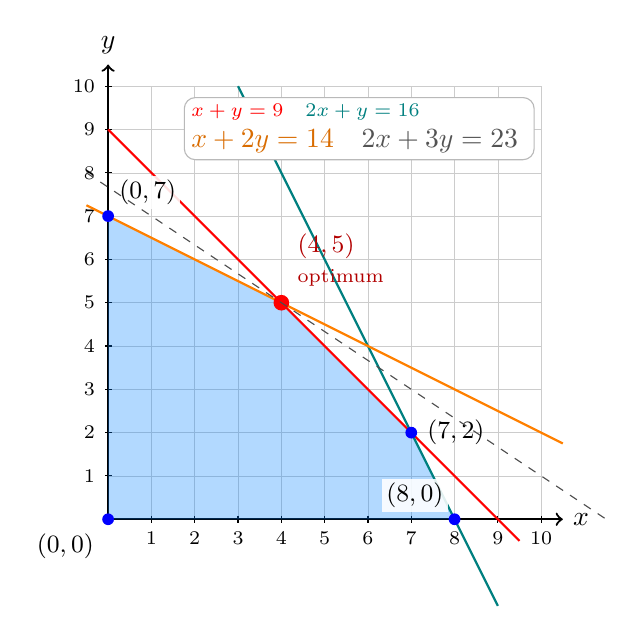
\begin{tikzpicture}[scale=0.55]
    % Grid and axes
    \draw[gray!40, very thin, step=1] (0,0) grid (10,10);
    \draw[->, thick] (0,0) -- (10.5,0) node[right] {$x$};
    \draw[->, thick] (0,0) -- (0,10.5) node[above] {$y$};
    \foreach \x in {1,...,10} \draw (\x,0.08) -- (\x,-0.08) node[below] {\scriptsize \x};
    \foreach \y in {1,...,10} \draw (0.08,\y) -- (-0.08,\y) node[left] {\scriptsize \y};

    % Feasible region: (0,0) -- (8,0) -- (7,2) -- (4,5) -- (0,7) -- cycle
    \fill[blue!50!cyan, opacity=0.3]
        (0,0) -- (8,0) -- (7,2) -- (4,5) -- (0,7) -- cycle;

    % Constraint boundary lines, extended a bit beyond the polygon
    % x + y = 9 (red): from (0,9) to (9,0)
    \draw[red, thick] (0,9) -- (9.5,-0.5);
    % 2x + y = 16 (teal): from (0,16) clipped, take (3,10) to (9,-2)
    \draw[teal, thick] (3,10) -- (9,-2);
    % x + 2y = 14 (orange): from (0,7) to (14,0)
    \draw[orange, thick] (-0.5,7.25) -- (10.5,1.75);

    % A compact legend keeps the four equations readable without stacking
    % labels on the nearby vertices and on one another.
    \node[anchor=north east, draw=gray!55, rounded corners,
          fill=white, inner sep=2.5pt, align=left] at (9.85,9.75) {
        \scriptsize\color{red}$x+y=9$\quad
        \color{teal}$2x+y=16$\\[-1pt]
        \color{orange!85!black}$x+2y=14$\quad
        \color{gray!65!black}$2x+3y=23$
    };

    % Vertices
    \node[fill=blue,circle,inner sep=1.5pt,label={below left:\small$(0,0)$}]   at (0,0) {};
    \node[fill=blue,circle,inner sep=1.5pt] at (8,0) {};
    \node[anchor=south east, fill=white, fill opacity=0.88,
          text opacity=1, inner sep=1.5pt] at (7.85,0.15) {\small$(8,0)$};
    \node[fill=blue,circle,inner sep=1.5pt,label={right:\small$(7,2)$}]        at (7,2) {};
    \node[fill=red, circle,inner sep=2pt] at (4,5) {};
    \node[anchor=south west, align=left, text=red!70!black]
        at (4.15,5.15) {\small $(4,5)$\\[-1pt]\scriptsize optimum};
    \node[fill=blue,circle,inner sep=1.5pt] at (0,7) {};
    \node[anchor=south west, fill=white, fill opacity=0.88,
          text opacity=1, inner sep=1.5pt] at (0.15,7.15) {\small$(0,7)$};

    % Optimal point and objective level set 2x + 3y = 23 (dashed)
    % line passes through (4,5): 8 + 15 = 23. Endpoints: (11.5,0) and (-0.5, 8)
    \draw[dashed, gray!60!black] (-0.5,8) -- (11.5,0);
\end{tikzpicture}
\end{center}
Untuk mengonversi pertidaksamaan ini menjadi persamaan, kita memperkenalkan variabel slack \(s_1\), \(s_2\), dan \(s_3\). Secara khusus, kita menulis ulang setiap kendala sebagai berikut:

\[
\begin{aligned}
x + y + s_1 &= 9, \\
2x + y + s_2 &= 16, \\
x + 2y + s_3 &= 14,
\end{aligned}
\]
dengan kendala nonnegativitas tambahan \(s_1, s_2, s_3 \ge 0\). 

Dengan demikian, program linier dalam bentuk standar menjadi:
\begin{tcolorbox}[
    colback=gray!5!white,
    colframe=gray!75!black,
    title=\textbf{Bentuk Standar},
    width=0.6\textwidth, % sesuaikan lebar sesuai keinginan
    box align=center
]
\[
\begin{aligned}
\max\quad 
& 2x + 3y \\
\st\quad 
& x + y + s_1 = 9, \\
& 2x + y + s_2 = 16, \\
& x + 2y + s_3 = 14, \\
& x, y, s_1, s_2, s_3 \ge 0.
\end{aligned}
\]
\end{tcolorbox}

\subsection*{Menulis Ulang Sistem dengan \(\{s_1,s_2,s_3\}\) sebagai Basis}

Ketika kita mengatakan bahwa \(\{s_1,s_2,s_3\}\) adalah basis, kita menyelesaikan setiap persamaan terhadap variabel slack yang bersesuaian:
\[
\begin{aligned}
s_1 &= 9 \;-\; x \;-\; y, \\[6pt]
s_2 &= 16 \;-\; 2x \;-\; y,\\[6pt]
s_3 &= 14 \;-\; x \;-\; 2y.
\end{aligned}
\]
 Variabel nonbasis awal kita adalah $x$ dan $y$. 
Kita akan menyebut representasi program linier ini sebagai suatu \emph{kamus}. 
\begin{tcolorbox}[colback=blue!5!white, colframe=blue!75!black,     width=0.6\textwidth, % sesuaikan lebar sesuai keinginan
    box align=center, title=\textbf{Kamus Awal}]
\[
\begin{aligned}
\max\quad 
& z = 0 + 2x + 3y \\
\st\quad 
& s_1 = 9 - x - y, \\
& s_2 = 16 - 2x - y, \\
& s_3 = 14 - x - 2y , \\
& x, y, s_1, s_2, s_3 \ge 0.
\end{aligned}
\]
Dari sini kita dapat membaca suatu \emph{solusi basis}, yaitu 
$$
\text{Variabel basis: } \ \ (s_1, s_2, s_3) = (9, 16,14),$$
$$
 \text{Variabel nonbasis:  } \ \ (x,y) = (0,0)
$$
dengan 
$$
\text{Nilai objektif: } z = 0.
$$
Karena semua variabel basis nonnegatif $(\geq 0)$, kita menyebutnya suatu \emph{solusi basis layak}.
\end{tcolorbox}

\begin{remark}{Membaca Kamus}{}
Dari kamus di bawah ini, kita dapat membaca \textbf{solusi basis} dan \textbf{nilai fungsi objektif} yang bersesuaian. Solusi basis diperoleh dengan:
\begin{itemize}
    \item Menetapkan semua \textbf{variabel nonbasis} (yang berada di ruas kanan persamaan, yaitu \(x\) dan \(y\)) sama dengan nol.
    \item Membaca nilai \textbf{variabel basis} (\(s_1, s_2, s_3\)) dari konstanta ruas kanan.
\end{itemize}

Kamus disebut \textbf{layak} jika semua variabel basis memiliki nilai nonnegatif (seperti yang berlaku di sini). Jadi, ini berkorespondensi dengan suatu solusi basis \emph{layak}:
\[
x = 0, \quad y = 0, \quad s_1 = 9, \quad s_2 = 16, \quad s_3 = 14, \quad z = 0.
\]
\vspace{1cm}

\[
\begin{aligned}
\max \quad 
& \tikzmark{zstart} \text{\colorbox{green!20!white}{$z = 0$\phantom{$1_1$}}} ~ \text{\colorbox{gray!20!white}{$+ 2\tikzmark{x1}x + 3\tikzmark{y1}y \tikzmark{zend}$}} \\
\st \quad 
& \tikzmark{s1start} \text{\colorbox{yellow}{$s_1 = 9$\phantom{1}}} ~ \tikzmark{s1rhs}\text{\colorbox{gray!20!white}{$- x - y$}} \tikzmark{s1end}, \\
& \tikzmark{s2start} \text{\colorbox{yellow}{$s_2 = 16$}} ~ \tikzmark{s2rhs} \text{\colorbox{gray!20!white}{$- 2x - y$}} \tikzmark{s2end}, \\
& \tikzmark{s3start} \text{\colorbox{yellow}{$s_3 = 14$}} ~ \tikzmark{s3rhs} \text{\colorbox{gray!20!white}{$- x - 2y$}} \tikzmark{s3end}, \\
& x, y, s_1, s_2, s_3 \ge 0.
\end{aligned}
\]

\begin{tikzpicture}[remember picture, overlay, >=stealth]

% Blue arrows: Basic variables and values
\draw[->, thick, blue] 
  ($(pic cs:s1rhs)+(-0.8,-0.1)$) -- ++(-3.5,-0.4) node[left, blue] {Variabel basis: $s_1 = 9$};
\draw[->, thick, blue] 
  ($(pic cs:s2rhs)+(-0.8,-0.10)$) -- ++(-3.5,-0.4) node[left, blue] {Variabel basis: $s_2 = 16$};
\draw[->, thick, blue] 
  ($(pic cs:s3rhs)+(-0.8,-0.10)$) -- ++(-3.5,-0.4) node[left, blue] {Variabel basis: $s_3 = 14$};

% Green arrow: Initial objective
\draw[->, thick, green!60!black] 
  ($(pic cs:zstart)+(0,0.1)$) -- ++(-2.5,1.0) node[left, green!50!black] {Objektif awal: $z = 0$};

% Red arrows: Non-basic variables
\draw[->, thick, red] 
  ($(pic cs:x1)+(0,0.3)$) -- ++(1.2,1.2) node[right, red] {Nonbasis: $x = 0$};
\draw[->, thick, red] 
  ($(pic cs:y1)+(0,0.3)$) -- ++(0.7,0.7) node[right, red] {Nonbasis: $y = 0$};

\end{tikzpicture}
\end{remark}

  

\subsection{Simpleks dengan Asumsi Titik Awal Layak}

Dalam subbagian ini, kita mengasumsikan bahwa basis slack \(\{s_1, s_2, s_3\}\) memberikan
kamus awal yang layak; yaitu, menetapkan variabel semula
\(x,y\) sama dengan nol menghasilkan nilai nonnegatif untuk setiap slack. Dengan
asumsi ini, metode simpleks berjalan dengan berulang kali memilih suatu
\emph{variabel masuk} yang koefisiennya pada baris objektif positif,
melakukan \emph{uji rasio} untuk memutuskan variabel basis mana yang keluar, dan
melakukan \emph{pivot} untuk memperoleh kamus baru. Bagian selanjutnya dari bagian ini
menguraikan ketiga langkah tersebut pada contoh berjalan di atas.

Kita mengambil sebagai variabel basis \emph{awal} ketiga variabel slack \(s_1, s_2, s_3\). Secara geometris, ini berkorespondensi dengan titik \(\,(x,y)=(0,0)\). Memang, jika \(x=0\) dan \(y=0\), maka dari kendala semula
\[
\begin{aligned}
  x + y + s_1 &= 9,\\
  2x + y + s_2 &= 16,\\
  x + 2y + s_3 &= 14,
\end{aligned}
\]
diperoleh bahwa
\[
s_1 = 9,
\quad
s_2 = 16,
\quad
s_3 = 14.
\]
Semuanya nonnegatif, sehingga \(\,(s_1,s_2,s_3)\) memang merupakan basis layak, dan \((0,0,9,16,14)\) merupakan \emph{solusi basis layak} (BFS).

Jadi, dalam bentuk ``variabel basis \(=\) konstanta \(-\) (suku nonbasis)'', sistem kita menjadi
\[
\begin{cases}
s_1 + x + y \;=\; 9,\\
s_2 + 2x + y \;=\; 16,\\
s_3 + x + 2y \;=\; 14.
\end{cases}
\]
Karena \(s_1, s_2, s_3\) diambil sebagai variabel \emph{basis}, variabel \emph{nonbasis} dalam susunan ini adalah \(x\) dan \(y\). Menetapkan \(x=0,\,y=0\) langsung memberikan BFS
\[
\bigl(x,y,s_1,s_2,s_3\bigr)
\;=\;
(0,\,0,\,9,\,16,\,14).
\]

\subsection*{Fungsi Objektif dalam Basis Ini}
%
%Fungsi objektif kita adalah:
\[
\max\quad z \;=\; 2x \;+\; 3y.
\]
%Perhatikan bahwa dalam basis saat ini, variabel slack tidak muncul pada baris objektif (koefisien biayanya nol), sehingga tidak ada suku tambahan yang melibatkan \(s_1\), \(s_2\), atau \(s_3\) pada persamaan \((z)\).
%
%Dengan demikian, jika semua persamaan dikumpulkan dalam format sederhana yang ``ramah kamus'':
%
%\[
%\begin{aligned}
%&z = 0 \;+\; 2x \;+\; 3y,
%&s_1 \;+\; x \;+\; y \quad\;=\quad 9,\\
%&s_2 \;+\; 2x \;+\; y \quad=\quad 16,\\
%&s_3 \;+\; x \;+\; 2y \;=\; 14,\\
%\end{aligned}
%\]
%dengan kendala nonnegativitas
%\[
%x,\,y,\,s_1,\,s_2,\,s_3 \;\ge\;0.
%\]
%
\paragraph{Nilai \(\,z\) pada BFS \(\,(0,0,9,16,14)\).}
%Pada \(\,(x,y)=(0,0)\), kita melihat \(z=2\cdot 0 + 3\cdot 0=0\). Jadi, nilai fungsi objektif awal adalah
%\[
%z=0.
%\]
Pada \((x,y)=(0,0)\), kita melihat \(z=2\cdot 0 + 3\cdot 0=0\), sehingga nilai
fungsi objektif awal adalah \(z=0\). Dari sini, biasanya kita melanjutkan dengan
\emph{pivot simpleks} untuk menaikkan fungsi objektif (karena ini adalah
masalah maksimisasi). Langkah-langkah pivot tersebut kita bahas berikutnya.
%
%Kita mulai dari BFS awal ketika \(\{s_1,s_2,s_3\}\) adalah variabel basis dan \(\{x,y\}\) adalah variabel nonbasis.
%Sistem pada tahap tersebut (dengan \(\,z = 2x + 3y\)) adalah:
%
%\[
%\begin{cases}
%s_1 = 9 \;-\; x \;-\; y,\\[4pt]
%s_2 = 16 \;-\; 2x \;-\; y,\\[4pt]
%s_3 = 14 \;-\; x \;-\; 2y,\\[4pt]
%z \;-\; 2x \;-\; 3y = 0.
%\end{cases}
%\]

\subsection*{Memilih Variabel Masuk}
\begin{tcolorbox}[colback=algenter!6, colframe=algenter, coltitle=white, fonttitle=\bfseries, sharp corners, title={\ding{43}\ Variabel Masuk}]

Kita memeriksa \emph{baris objektif} untuk menentukan variabel nonbasis mana yang harus masuk ke basis. Pada tahap ini, fungsi objektifnya adalah:
\[
z = 2x + 3y.
\]

\begin{itemize}
  \item Variabel nonbasis adalah \(x\) dan \(y\).
  \item Keduanya memiliki koefisien \textbf{positif}, yang berarti bahwa meningkatkan salah satu variabel (sambil mempertahankan kelayakan) akan meningkatkan nilai fungsi objektif \(z\).
  \item Untuk memilih di antara keduanya, kita menerapkan suatu \textbf{aturan pivot}, yaitu strategi untuk memilih di antara variabel masuk yang memenuhi syarat.
  
  \textbf{Dalam contoh ini, kita menggunakan aturan \emph{Pendakian Tercuram}: kita memilih variabel nonbasis dengan koefisien positif terbesar pada baris objektif.}
  
  \item Di antara \(x\) dan \(y\), koefisien \(y\) lebih besar (\(3 > 2\)).
\end{itemize}

Oleh karena itu, kita memilih \(\boxed{y}\) untuk \textbf{masuk} ke basis.

\end{tcolorbox}

\subsubsection*{Iterasi Pertama. Uji Rasio untuk Menentukan Variabel yang Keluar}

\begin{tcolorbox}[colback=algleave!6, colframe=algleave, coltitle=white, fonttitle=\bfseries, sharp corners, title={\ding{47}\ Iterasi Pertama: Uji Rasio}]

Kita menahan \(x = 0\) tetap dan membiarkan \(y\) meningkat dari \(0\).  
Kemudian dari kamus awal, variabel basis menjadi (dengan menyubstitusikan \(x = 0\)):

\[
\begin{aligned}
s_1 &= 9 - y, \\
s_2 &= 16 - y, \\
s_3 &= 14 - 2y.
\end{aligned}
\]

Untuk mempertahankan kelayakan, kita mengharuskan semua variabel basis tetap nonnegatif:
\[
\begin{aligned}
s_1 \ge 0 &\;\implies\; 9 - y \ge 0 \;\implies\; y \le 9, \\
s_2 \ge 0 &\;\implies\; 16 - y \ge 0 \;\implies\; y \le 16, \\
s_3 \ge 0 &\;\implies\; 14 - 2y \ge 0 \;\implies\; y \le 14/2 = 7.
\end{aligned}
\]

\emph{Kendala paling ketat} adalah \(y \le 7\), yang berarti \(s_3\) mencapai nol terlebih dahulu ketika \(y\) meningkat.  
Oleh karena itu, \(\boxed{s_3}\) akan \textbf{keluar dari basis} pada pivot ini.

\end{tcolorbox}

Ini disebut \emph{Uji Rasio} karena kita dapat menghitung bilangan-bilangan tersebut sebagai 
$$
9 - y = 0 \quad \Rightarrow y = 9 / 1 = 9
$$

$$
16 - y = 0 \quad \Rightarrow y = 16 / 1 = 16
$$

$$
14 - 2y = 0 \quad \Rightarrow y = 14 / 2 = 7
$$

Jika koefisien pada $y$ positif, kita akan mengabaikan kendala tersebut karena meningkatkan $y$ tidak akan pernah melanggar pertidaksamaan yang bersesuaian.

Uji rasio juga dapat dipandang sebagai perubahan solusi melalui suatu vektor. Secara khusus, kita berada pada solusi basis layak $(s_1, s_2, s_3, x,y) = (9,16,14,0,0)$. Sekarang, ketika kita meningkatkan $y$, kita mengubah solusi sebagai 

\begin{align*}
 (s_1, s_2, s_3, x,y) &= (9,16,14,0,0) + \Delta y \cdot (-1, -1, -2, 0,1)\\
 &= (9,16,14,0,0) + 7\cdot (-1, -1, -2, 0,1)  = (2,9,0,0,7).
\end{align*}
Kita akan melihat bilangan-bilangan ini muncul ketika kita melakukan pivot kamus ke basis baru.

\subsection*{Melakukan Pivot pada Persamaan \(s_3\) yang Diselesaikan terhadap \(y\)}

Semula, \(s_3 + x + 2y = 14\). Selesaikan terhadap \(y\):
\[
y \;=\; 7 \;-\; \tfrac{x}{2} \;-\; \tfrac{s_3}{2}.
\]
Substitusikan ke baris-baris lain (dan baris objektif), dengan mengisolasi setiap variabel \emph{basis} di ruas kiri dan semua variabel lainnya di ruas kanan:
\[
\begin{aligned}
\max\quad 
& z = 0+ 2x + 3y \quad && = 21 + \frac{1}{2}x - \frac{3}{2}s_3 \\
\st\quad 
& s_1 = 9 - x - y \quad && = 2 - \frac{1}{2}x + \frac{1}{2}s_3, \\
& s_2 = 16 - 2x - y \quad &&= 9 - \frac{3}{2}x + \frac{1}{2}s_3, \\
& s_3 = 14 - x - 2y \quad \Rightarrow y &&= 7 - \frac{1}{2}x - \frac{1}{2}s_3, \\
& x, y, s_1, s_2, s_3 \ge 0.
\end{aligned}
\]

\noindent
Dengan demikian, variabel \emph{basis} yang baru adalah \(\{z,\,y,\,s_1,\,s_2\}\) jika kita juga menempatkan \(z\) di dalam kamus. Biasanya, dalam kamus simpleks standar, \(z\) ditampilkan pada baris tersendiri, tetapi tidak dihitung sebagai ``variabel basis'' dalam pengertian yang sama seperti kendala. Variabel nonbasis sekarang adalah \(\{x,\,s_3\}\).

\subsection*{Kamus dan Solusi Basis Layak yang Diperbarui}

\begin{tcolorbox}[colback=algpivot!6, colframe=algpivot, coltitle=white, fonttitle=\bfseries, sharp corners, title={\ding{114}\ Pivot: Kamus Kedua}]

\[
\begin{aligned}
\max\quad 
& z =  21 + \frac{1}{2}x - \frac{3}{2}s_3 \\
\st\quad 
& s_1  = 2 - \frac{1}{2}x + \frac{1}{2}s_3, \\
& s_2  = 9 - \frac{3}{2}x + \frac{1}{2}s_3, \\
& y = 7 - \frac{1}{2}x - \frac{1}{2}s_3, \\
& x, y, s_1, s_2, s_3 \ge 0.
\end{aligned}
\]

\begin{itemize}
  \item Tetapkan \(\,x=0\) dan \(\,s_3=0\) (variabel nonbasis baru). 
  \item Kemudian \(\,(y,s_1,s_2)\) menjadi:
  \[
  y = 7, 
  \quad
  s_1 = 2,
  \quad
  s_2 = 9.
  \]
  \item Substitusikan ke baris objektif:
  \[
  z = 21 + \tfrac12\cdot 0 - \tfrac32\cdot 0 \;=\; 21.
  \]
\end{itemize}
Jadi, BFS baru setelah pivot adalah 
\(\bigl(x,y,s_1,s_2,s_3\bigr) = \bigl(0,7,2,9,0\bigr)\) 
dengan \(z=21\).
\end{tcolorbox}

\subsection*{Iterasi Kedua}
Karena fungsi objektif masih memiliki variabel dengan koefisien positif, kita akan mencoba melakukan pivot lagi untuk meningkatkan fungsi objektif.

\subsubsection*{Iterasi Kedua. Mengidentifikasi Variabel Masuk}
\begin{tcolorbox}[colback=algenter!6, colframe=algenter, coltitle=white, fonttitle=\bfseries, sharp corners, title={\ding{43}\ Iterasi Kedua: Variabel Masuk}]
Kita melihat koefisien variabel nonbasis pada baris \emph{objektif},
\[
z = 21 \;+\; \tfrac12\,x \;-\;\tfrac32\,s_3.
\]
\begin{itemize}
  \item \(x\) memiliki koefisien \(\tfrac12\) (yang \textbf{positif}), 
  \item \(s_3\) memiliki koefisien \(-\tfrac32\) (negatif).
\end{itemize}
Karena ini adalah masalah \emph{maksimisasi}, meningkatkan suatu variabel dengan koefisien objektif \textbf{negatif} akan \emph{menurunkan} \(z\).  
Dengan demikian, kita memilih \(x\), satu-satunya variabel nonbasis dengan koefisien positif, untuk \emph{masuk} ke basis.
\end{tcolorbox}
\subsubsection*{Iterasi Kedua. Uji Rasio untuk Menentukan Variabel yang Keluar}

\begin{tcolorbox}[colback=algleave!6, colframe=algleave, coltitle=white, fonttitle=\bfseries, sharp corners, title={\ding{47}\ Iterasi Kedua: Uji Rasio}]

Untuk sementara, kita menahan \(s_3=0\) dan membiarkan \(x\) meningkat dari \(0\).  
Kemudian dari sistem di atas, ketiga variabel basis menjadi (dengan menyubstitusikan \(s_3=0\)):

\[
\begin{aligned}
y   &= 7 - \tfrac12\,x,\\
s_1 &= 2 - \tfrac12\,x,\\
s_2 &= 9 - \tfrac32\,x.
\end{aligned}
\]
Kita mengharuskan variabel-variabel ini tetap nonnegatif:
\[
\begin{aligned}
y \ge 0 \;&\implies\; 7 - \tfrac12\,x \;\ge\; 0 \;\implies\; x \;\le\; 7/\tfrac{1}{2} = 14,\\
s_1 \ge 0 \;&\implies\; 2 - \tfrac12\,x \;\ge\; 0 \;\implies\; x \;\le\; 2/\tfrac{1}{2} = 4,\\
s_2 \ge 0 \;&\implies\; 9 - \tfrac32\,x \;\ge\; 0 \;\implies\; x \;\le\; 9/\tfrac{3}{2} = 6.
\end{aligned}
\]
Batas atas \emph{terkecil} adalah \(x \le 4\), yang berarti \(\,s_1\) akan mencapai nol terlebih dahulu ketika \(x=4\).  
Dengan demikian, \(\,s_1\) harus \emph{keluar} dari basis.
\end{tcolorbox}
\subsubsection*{Pivot: Menyelesaikan Persamaan \(s_1\) terhadap \(x\)}

Dari
\[
s_1 = 2 \;-\;\tfrac12\,x \;+\;\tfrac12\,s_3,
\]
kita mengisolasi \(x\):
\[
s_1 - 2 - \tfrac12\,s_3 = -\,\tfrac12\,x
\quad\Longrightarrow\quad
x = -2\Bigl(s_1 - 2 - \tfrac12\,s_3\Bigr)
\;=\;
4 \;+\; s_3 \;-\; 2\,s_1.
\]
Dengan menulis ulang,
\[
x \;+\; 2\,s_1 \;-\; s_3 
\;=\;
4.
\]
Ini \emph{menjadi baris pivot baru}, dengan \(x\) di ruas kiri sebagai variabel basis.

\subsubsection*{Mengeliminasi \(x\) dari Baris Lain}

Selanjutnya, kita menyubstitusikan 
\(\;x = 4 + s_3 - 2\,s_1\;\)
ke dalam baris-baris untuk \(\{y,\,s_2,\,z\}\) guna menghilangkan \(x\).  
(Pada setiap baris, ganti \(x\) dengan \(\,4 + s_3 - 2\,s_1\).)

\paragraph{Memperbarui \(y\):}

Semula 
\[
y = 7 - \tfrac12\,x - \tfrac12\,s_3.
\]
Substitusikan \(x\):
\[
y
= 7 
- \tfrac12\bigl(4 + s_3 - 2s_1\bigr)
- \tfrac12\,s_3
=
7 - 2 - \tfrac12\,s_3 + s_1 - \tfrac12\,s_3
=
5 + s_1 - s_3.
\]
%Dengan demikian
%\[
%y
%\;-\;
%s_1
%\;+\;
%s_3
%\;=\;
%5.
%\]

\paragraph{Memperbarui \(s_2\):}

Semula
\[
s_2 = 9 - \tfrac32\,x + \tfrac12\,s_3.
\]
Substitusikan \(x\):
\[
s_2
= 9 
- \tfrac32\bigl(4 + s_3 - 2s_1\bigr)
+ \tfrac12\,s_3
= 
9 - 6 - \tfrac32\,s_3 + 3\,s_1 + \tfrac12\,s_3
=
3 + 3\,s_1 - s_3.
\]
%Dengan demikian
%\[
%s_2
%\;-\;
%3\,s_1
%\;+\;
%s_3
%\;=\;
%3.
%\]

\paragraph{Memperbarui Baris Objektif \(\,z\):}

Semula
\[
z = 21 + \tfrac12\,x - \tfrac32\,s_3.
\]
Substitusikan \(x\):
\[
z
= 
21 
+ \tfrac12\bigl(4 + s_3 - 2s_1\bigr)
- \tfrac32\,s_3
=
21 + 2 + \tfrac12\,s_3 - s_1 - \tfrac32\,s_3
=
23 - s_1 - s_3.
\]
%Atau
%\[
%z
%\;+\;
%s_1
%\;+\;
%s_3
%\;=\;
%23.
%\]

\subsection*{Kamus Ketiga}

\begin{tcolorbox}[colback=algopt!6, colframe=algopt, coltitle=white, fonttitle=\bfseries, sharp corners, title={\ding{52}\ Optimal: Kamus Akhir}]

Setelah pivot, variabel basis sekarang adalah
\(\,\{\,x,\,y,\,s_2\}\), 
dan variabel nonbasis adalah 
\(\,\{\,s_1,\,s_3\}\).  
Persamaan kita yang telah diperbarui, dalam bentuk kamus yang rapi (variabel basis di ruas kiri), adalah:

\[
\begin{aligned}
\max\quad 
& z = 23 - s_1 - s_3 \\
\st\quad 
& x = 4 - 2s_1 + s_3, \\
& y = 5 + s_1 - s_3, \\
& s_2 = 3 + 3s_1 - s_3, \\
& x, y, s_1, s_2, s_3 \geq 0.
\end{aligned}
\]

\begin{itemize}
  \item Menetapkan variabel nonbasis baru \(\,s_1=0\) dan \(\,s_3=0\) memberikan
  \[
  x=4, \quad y=5,\quad s_2=3,\quad z=23.
  \]
  \item Jadi, BFS baru kita adalah 
  \(\bigl(x,y,s_1,s_2,s_3\bigr)=\bigl(4,\,5,\,0,\,3,\,0\bigr)\) 
  dengan nilai fungsi objektif \(z=23\).
\end{itemize}
\end{tcolorbox}

\begin{remark}{Membaca Kamus Akhir}{}
Dari kamus akhir di bawah ini, kita membaca solusi menggunakan proses yang sama:
\begin{itemize}
    \item Tetapkan semua \textbf{variabel nonbasis} sama dengan nol. Di sini, variabel nonbasis adalah \(s_1\) dan \(s_3\).
    \item Hitung nilai variabel basis \(x, y, s_2\) dan fungsi objektif \(z\).
\end{itemize}

Ini menghasilkan solusi basis layak akhir:
\[
s_1 = 0, \quad s_3 = 0, \quad x = 4, \quad y = 5, \quad s_2 = 3, \quad z = 23.
\]

\[
\begin{aligned}
\max \quad 
& \text{\colorbox{green!20!white}{$z = 23$}} ~ \text{\colorbox{gray!20!white}{$- s_1 - s_3$}} \\
\st \quad 
& \text{\colorbox{yellow}{$x = 4$}} ~ \text{\colorbox{gray!20!white}{$- 2s_1 + s_3$}}, \\
& \text{\colorbox{yellow}{$y = 5$}} ~ \text{\colorbox{gray!20!white}{$+ s_1 - s_3$}}, \\
& \text{\colorbox{yellow}{$s_2 = 3$}} ~ \text{\colorbox{gray!20!white}{$+ 3s_1 - s_3$}}, \\
& x, y, s_1, s_2, s_3 \ge 0.
\end{aligned}
\]

\begin{center}
\small
\begin{tabular}{@{}ll@{}}
\textcolor{green!50!black}{Objektif akhir} & \(z=23\) \\
\textcolor{blue}{Variabel basis} & \(x=4,\ y=5,\ s_2=3\) \\
\textcolor{red}{Variabel nonbasis} & \(s_1=0,\ s_3=0\)
\end{tabular}
\end{center}

\textbf{Mengapa solusi ini optimal?}  
Ini adalah masalah maksimisasi, dan kamus akhir menyatakan fungsi objektif sebagai:
\[
z = 23 - s_1 - s_3.
\]
Baik \(s_1\) maupun \(s_3\) merupakan variabel nonbasis dan saat ini bernilai nol. Karena meningkatkan salah satunya akan \emph{menurunkan} nilai \(z\), kita tidak dapat memperbaiki fungsi objektif melalui pivot.  
\\[0.5em]
\textbf{Dengan demikian, solusi ini optimal.}
\end{remark}

\subsection{Merangkum langkah-langkah yang dilakukan}
Sekarang kita merangkum seluruh proses:

\begin{enumerate}
    \item \textbf{PL Semula}  
    \begin{tcolorbox}[colback=orange!5!white, colframe=orange!75!black,    
    width=0.6\textwidth, % sesuaikan lebar sesuai keinginan
    box align=center, 
    title=\textbf{Program Linier yang Akan Diselesaikan}]
    \[
    \begin{aligned}
    \max \quad & 2x + 3y \\
    \st \quad 
    & x + y \leq 9, \\
    & 2x + y \leq 16, \\
    & x + 2y \leq 14, \\
    & x, y \geq 0.
    \end{aligned}
    \]
    \end{tcolorbox}

    \item \textbf{Bentuk Standar dengan Basis Layak $\{s_1, s_2, s_3\}$}  
    \begin{tcolorbox}[colback=gray!5!white, colframe=gray!75!black,    
    width=0.6\textwidth, % sesuaikan lebar sesuai keinginan
    box align=center, 
    title=\textbf{Bentuk Standar}]
    \[
    \begin{aligned}
    \max \quad & 2x + 3y \\
    \st \quad 
    & x + y + s_1 = 9, \\
    & 2x + y + s_2 = 16, \\
    & x + 2y + s_3 = 14, \\
    & x, y, s_1, s_2, s_3 \geq 0.
    \end{aligned}
    \]
    \end{tcolorbox}

    \item \textbf{Kamus Awal dengan Basis \( (s_1, s_2, s_3) \)}
    \begin{tcolorbox}[colback=blue!5!white, colframe=blue!75!black,    
    width=0.6\textwidth, % sesuaikan lebar sesuai keinginan
    box align=center, 
    title=\textbf{Kamus Awal}]
    \[
    \begin{aligned}
    \max \quad & z = 0 + 2x + 3y \\
    \st \quad 
    & s_1 = 9 - x - y, \\
    & s_2 = 16 - 2x - y, \\
    & s_3 = 14 - x - 2y.\\
    & x,y,s_1, s_2, s_3 \geq 0
    \end{aligned}
    \]
    \end{tcolorbox}
    Solusi Basis Layak: \( (s_1, s_2, s_3) = (9,16,14), (x,y) = (0,0) \)  
    Nilai Fungsi Objektif: \( z = 0 \).\\  
    Karena baris objektif memiliki koefisien positif, solusi ini belum optimal.
    
    \item \textbf{Iterasi Pertama:}
\begin{enumerate}
    \item \textbf{Uji Rasio:} \( y \) masuk, \( s_3 \) keluar.

    \item \textbf{Kamus setelah Pivot dengan \( y \) masuk dan \( s_3 \) keluar}  
    \begin{tcolorbox}[colback=blue!5!white, colframe=blue!75!black,    
    width=0.6\textwidth, % sesuaikan lebar sesuai keinginan
    box align=center, 
    title=\textbf{Kamus Kedua}]
    \[
    \begin{aligned}
    \max \quad & z = 21 + \frac{1}{2}x - \frac{3}{2}s_3 \\
    \st \quad 
    & s_1 = 2 - \frac{1}{2}x + \frac{1}{2}s_3, \\
    & s_2 = 9 - \frac{3}{2}x + \frac{1}{2}s_3, \\
    & y = 7 - \frac{1}{2}x - \frac{1}{2}s_3.
    \end{aligned}
    \]
    \end{tcolorbox}
    Solusi Basis Layak: \( (s_1, s_2, y) = (2,9,7), (x,s_3) = (0,0) \)  
    Nilai Fungsi Objektif: \( z = 21 \).\\ 
    Karena baris objektif memiliki koefisien positif, solusi ini belum optimal.  
    \end{enumerate}
    \item \textbf{Iterasi Kedua}
    \begin{enumerate}
    \item \textbf{Uji Rasio:} \( x \) masuk, \( s_1 \) keluar.

    \item \textbf{Kamus Akhir (Optimal) setelah pivot dengan $x$ masuk dan $s_1$ keluar.} 
    \begin{tcolorbox}[colback=green!5!white, colframe=green!75!black,    
    width=0.6\textwidth, % sesuaikan lebar sesuai keinginan
    box align=center, 
    title=\textbf{Kamus Akhir}] 
    \[
    \begin{aligned}
    \max \quad & z = 23 - s_1 - s_3 \\
    \st \quad
    & x = 4 - 2s_1 + s_3, \\
    & y = 5 + s_1 - s_3, \\
    & s_2 = 3 + 3s_1 - s_3.
    \end{aligned}
    \]
    \end{tcolorbox}
    Solusi Basis Layak: \( (x,y,s_2) = (4,5,3), (s_1,s_3) = (0,0) \)  
    Nilai Fungsi Objektif: \( z = 23 \).\\ 
    Karena semua koefisien pada baris objektif nonpositif, inilah solusi optimal.
    \end{enumerate}
\end{enumerate}

\begin{resource}
Anda dapat meninjau perhitungan ini menggunakan kode dalam format Jupyter Notebook yang tersedia di sini.
\begin{itemize}
\item \href{https://colab.research.google.com/drive/1kUWeNOVZByIoSWWUEUEFwwdFhAQvGcsG?usp=sharing}{Versi Colab (daring)}
\item \href{https://github.com/open-optimization/open-optimization-or-examples/blob/master/linear-programming/Simplex_Tableaus_From_Basis.ipynb}{Jupyter Notebook untuk Diunduh}
\end{itemize}
\end{resource}

Cara yang berguna untuk menghayati apa yang baru saja terjadi: \emph{setiap titik sudut daerah layak memiliki kamusnya sendiri}, yaitu program linier yang sama ditulis ulang dari sudut pandang titik sudut tersebut. Gambar~\ref{fig:bfs-perspectives} menunjukkan kelima kamus untuk contoh kita. Metode simpleks cukup berjalan dari satu kamus ke kamus lain sepanjang sisi-sisi daerah, dan tanda koefisien baris objektif pada setiap titik sudut menunjukkan arah selanjutnya. Pada $(4,5)$ kedua koefisien negatif, sehingga perjalanan berhenti: tidak ada titik sudut tetangga yang lebih baik.

\begin{figure}[h!]
\begin{center}
\begin{tikzpicture}[scale=0.5,
    dictbox/.style={draw=black!60, fill=white, rounded corners=2pt, inner sep=3pt, font=\scriptsize},
    optbox/.style={draw=green!60!black, thick, fill=green!5, rounded corners=2pt, inner sep=3pt, font=\scriptsize},
    connect/.style={black!35, thin}]
    % Grid and axes
    \draw[gray!40, very thin, step=1] (0,0) grid (10,10);
    \draw[->, thick] (0,0) -- (10.5,0) node[right] {$x$};
    \draw[->, thick] (0,0) -- (0,10.5) node[above] {$y$};
    \foreach \x in {2,4,6,8,10} \draw (\x,0.08) -- (\x,-0.08) node[below] {\scriptsize \x};
    \foreach \y in {2,4,6,8,10} \draw (0.08,\y) -- (-0.08,\y) node[left] {\scriptsize \y};

    % Feasible region: (0,0) -- (8,0) -- (7,2) -- (4,5) -- (0,7) -- cycle
    \fill[blue!50!cyan, opacity=0.3] (0,0) -- (8,0) -- (7,2) -- (4,5) -- (0,7) -- cycle;
    \draw[blue!60!black, thick] (0,0) -- (8,0) -- (7,2) -- (4,5) -- (0,7) -- cycle;

    % Simplex path taken in the text: (0,0) -> (0,7) -> (4,5)
    \draw[->, very thick, orange!90!black] (0,0.35) -- (0,6.6);
    \draw[->, very thick, orange!90!black] (0.35,6.72) -- (3.6,5.32);

    % Vertices
    \foreach \p in {(0,0),(8,0),(7,2),(4,5),(0,7)} \node[blue] at \p [circle,fill,inner sep=1.6pt]{};
    \node[green!50!black] at (4,5) [circle,draw,thick,inner sep=3pt]{};

    % Dictionary boxes
    \node[dictbox, anchor=north east] (d00) at (-2.2,3.2) {$\begin{aligned}[t]
        \textbf{(0,0)}:\ z &= 0 + 2x + 3y\\
        s_1 &= 9 - x - y\\
        s_2 &= 16 - 2x - y\\
        s_3 &= 14 - x - 2y
        \end{aligned}$};
    \node[dictbox, anchor=south east] (d07) at (-2.2,8.4) {$\begin{aligned}[t]
        \textbf{(0,7)}:\ z &= 21 + \tfrac12 x - \tfrac32 s_3\\
        s_1 &= 2 - \tfrac12 x + \tfrac12 s_3\\
        s_2 &= 9 - \tfrac32 x + \tfrac12 s_3\\
        y &= 7 - \tfrac12 x - \tfrac12 s_3
        \end{aligned}$};
    \node[optbox, anchor=south west] (d45) at (9.3,7.6) {$\begin{aligned}[t]
        \textbf{(4,5) optimal}:\ z &= 23 - s_1 - s_3\\
        x &= 4 - 2s_1 + s_3\\
        y &= 5 + s_1 - s_3\\
        s_2 &= 3 + 3s_1 - s_3
        \end{aligned}$};
    \node[dictbox, anchor=west] (d72) at (11.6,3.4) {$\begin{aligned}[t]
        \textbf{(7,2)}:\ z &= 20 - 4s_1 + s_2\\
        x &= 7 + s_1 - s_2\\
        y &= 2 - 2s_1 + s_2\\
        s_3 &= 3 + 3s_1 - s_2
        \end{aligned}$};
    \node[dictbox, anchor=north west] (d80) at (9.3,-1.2) {$\begin{aligned}[t]
        \textbf{(8,0)}:\ z &= 16 + 2y - s_2\\
        x &= 8 - \tfrac12 y - \tfrac12 s_2\\
        s_1 &= 1 - \tfrac12 y + \tfrac12 s_2\\
        s_3 &= 6 - \tfrac32 y + \tfrac12 s_2
        \end{aligned}$};

    % Connectors from boxes to vertices
    \draw[connect] (d00.east) -- (0,0);
    \draw[connect] (d07.east) -- (0,7);
    \draw[connect] (d45.south west) -- (4,5);
    \draw[connect] (d72.west) -- (7,2);
    \draw[connect] (d80.north west) -- (8,0);

    % Objective value table
    \node[draw=black!60, fill=white, anchor=north, font=\scriptsize] at (3.5,-2.2) {
        \begin{tabular}{c|ccccc}
        vertex & $(0,0)$ & $(8,0)$ & $(7,2)$ & $(4,5)$ & $(0,7)$\\
        \hline
        $z$ & $0$ & $16$ & $20$ & $\mathbf{23}$ & $21$
        \end{tabular}};
\end{tikzpicture}
\end{center}
\caption{Program linier yang sama dilihat dari setiap titik sudut: setiap solusi basis layak memiliki kamusnya sendiri, dan baris objektifnya mengungkapkan apakah terdapat tetangga yang lebih baik. Panah jingga menelusuri pivot yang dilakukan dalam teks, $(0,0) \to (0,7) \to (4,5)$; pada $(4,5)$ semua koefisien objektif negatif, yang membuktikan optimalitas.}
\label{fig:bfs-perspectives}
\end{figure}

\section{Algoritma Simpleks!}
\label{sec:simplex-algorithm}
Di sini kita menjelaskan algoritma simpleks secara formal.
\begin{algocard}{Algoritma: Metode Simpleks}
\textbf{Masukan.} Suatu program linier berbentuk standar dengan basis awal yang layak (biasanya variabel slack).\\
\textbf{Inisialisasi.} Tuliskan sistem dalam bentuk kamus (variabel basis di ruas kiri, variabel nonbasis di ruas kanan) dan substitusikan variabel basis ke dalam fungsi objektif.
\algostep{algenter}{\ding{43}}{Pilih variabel masuk}{Pilih variabel nonbasis dengan koefisien positif pada baris objektif. (Jika tidak ada koefisien positif, solusi saat ini sudah optimal.)}
\algostep{algleave}{\ding{47}}{Tentukan variabel keluar}{Untuk setiap variabel basis dengan koefisien variabel masuk positif, hitung rasio $\dfrac{\text{nilai variabel basis saat ini}}{\text{koefisien variabel masuk}}$. Variabel basis dengan rasio \emph{terkecil} mencapai nol terlebih dahulu dan keluar dari basis.}
\algostep{algpivot}{\ding{114}}{Pivot}{Tuliskan ulang persamaan variabel keluar agar dinyatakan terhadap variabel masuk, lalu substitusikan ekspresi ini ke semua persamaan lain dan fungsi objektif.}
\algostep{algopt}{\ding{52}}{Ulangi hingga optimal}{Ulangi ketiga langkah di atas sampai setiap koefisien baris objektif dari variabel nonbasis bernilai nonpositif. Solusi basis saat ini kemudian \textbf{optimal}.}
\end{algocard}

Di sini kita mendalami sedikit lagi apa yang dimaksud dengan uji rasio:
\begin{itemize}
    \item \textbf{Uji Rasio (Definisi Formal)}  

    Uji Rasio digunakan untuk menentukan variabel basis mana yang harus keluar dari basis ketika suatu variabel nonbasis masuk. Uji ini memastikan bahwa kita mempertahankan kelayakan dengan mencegah variabel basis menjadi negatif.

    Dengan suatu \emph{kolom pivot} yang berkorespondensi dengan variabel masuk (misalnya, \( x_e \)), Uji Rasio didefinisikan sebagai berikut:

    \begin{itemize}
        \item Identifikasi semua kendala berbentuk:
        \[
        s_i = b_i - a_{i,e} x_e
        \]
        dengan \( b_i \) adalah nilai ruas kanan, dan \( a_{i,e} \) adalah koefisien variabel masuk pada baris \( i \).
        \item Hitung rasio untuk semua kendala dengan \( a_{i,e} > 0 \):
        \[
        \frac{b_i}{a_{i,e}}
        \]
        \item \emph{Variabel keluar} berkorespondensi dengan baris yang menghasilkan \emph{rasio positif terkecil}. Ini memastikan bahwa peningkatan \( x_e \) tidak menyebabkan variabel basis menjadi negatif.
    \end{itemize}

    \textbf{Kasus Khusus:}
    \begin{itemize}
        \item Jika semua \( a_{i,e} \leq 0 \), maka masalah \emph{tak terbatas}, yang berarti fungsi objektif dapat ditingkatkan tanpa batas.
        \item Jika beberapa baris mencapai rasio minimum yang sama, diperlukan \emph{aturan pemecah hasil imbang} (misalnya, Aturan Bland untuk menghindari siklus).
    \end{itemize}

    Uji Rasio menjamin bahwa kita selalu memilih kendala yang tepat untuk mempertahankan kelayakan selama melakukan pivot menuju solusi yang lebih baik.
\end{itemize}

\begin{learningcheckpoint}[label={lc:ratio-test}]
Ketika menerapkan metode simpleks, mengapa pemilihan variabel keluar yang salah selama uji rasio dapat menghasilkan solusi basis yang \emph{tidak layak}?

\emph{Petunjuk: Pikirkan apa yang hendak dijamin oleh uji rasio bagi nonnegativitas variabel setelah pivot.}
\end{learningcheckpoint}

Kita akan melihat contoh lain tentang hal ini, lalu memodifikasinya untuk menangani PL yang tidak memiliki solusi basis layak awal yang sederhana.

\subsection{Eksekusi Algoritma Simpleks}

Berikut adalah perhitungan yang sama dari Bagian~\ref{sec:pivoting}, kali ini dalam bentuk ringkas, sehingga Anda dapat melihat seluruh proses secara sekilas setelah setiap langkah memiliki nama. Setiap perhitungan diberi kode warna yang sesuai dengan kartu algoritma di atas: {\color{algenter}\textbf{masuk}} (hijau), {\color{algleave}\textbf{uji rasio / keluar}} (jingga), {\color{algpivot}\textbf{pivot}} (biru), dan {\color{algopt}\textbf{optimal}} (ungu).

\noindent\textbf{Kamus awal} (basis \(\{s_1,s_2,s_3\}\); nonbasis \(x=y=0\)):
\[
\begin{aligned}
\max\quad & z = 2x + 3y \\
\st\quad  & s_1 = 9 - x - y \\
          & s_2 = 16 - 2x - y \\
          & s_3 = 14 - x - 2y
\end{aligned}
\]

\noindent\textbf{Iterasi 1.}
\begin{steppanel}{algenter}
\slab{algenter}{43}{Masuk} Baik \(x\) maupun \(y\) memiliki koefisien positif dalam \(z = 2x + 3y\). Berdasarkan pendakian tercuram, kita meningkatkan variabel dengan koefisien lebih besar, yaitu \(y\) (koefisien \(3\)), sehingga \(y\) \textbf{masuk}.
\end{steppanel}
\begin{steppanel}{algleave}
\slab{algleave}{47}{Uji rasio} Ketika \(y\) meningkat (dengan \(x=0\)), setiap variabel basis tetap nonnegatif hanya sampai rasionya:
\[
\begin{aligned}
s_1 = 9 - y   &\ge 0 \iff y \le 9/1  = 9,\\
s_2 = 16 - y  &\ge 0 \iff y \le 16/1 = 16,\\
s_3 = 14 - 2y &\ge 0 \iff y \le 14/2 = 7 \quad(\text{terkecil}).
\end{aligned}
\]
Rasio terkecil adalah \(7\), yang dicapai oleh \(s_3\), sehingga \(s_3\) \textbf{keluar}.
\end{steppanel}
\begin{steppanel}{algpivot}
\slab{algpivot}{114}{Pivot} Selesaikan baris \(s_3\) terhadap \(y\): \(y = 7 - 0.5x - 0.5s_3\). Menyubstitusikannya ke fungsi objektif dan baris-baris lain memberikan
\[
\begin{aligned}
\max\quad & z = 21 + 0.5x - 1.5s_3 \\
\st\quad  & s_1 = 2 - 0.5x + 0.5s_3 \\
          & s_2 = 9 - 1.5x + 0.5s_3 \\
          & y = 7 - 0.5x - 0.5s_3
\end{aligned}
\]
\end{steppanel}

\noindent\textbf{Iterasi 2.}
\begin{steppanel}{algenter}
\slab{algenter}{43}{Masuk} Hanya \(x\) yang memiliki koefisien objektif positif (\(0.5\)), sehingga \(x\) \textbf{masuk}.
\end{steppanel}
\begin{steppanel}{algleave}
\slab{algleave}{47}{Uji rasio} Ketika \(x\) meningkat (dengan \(s_3=0\)):
\[
\begin{aligned}
s_1 = 2 - 0.5x &\ge 0 \iff x \le 2/0.5 = 4 \quad(\text{terkecil}),\\
s_2 = 9 - 1.5x &\ge 0 \iff x \le 9/1.5 = 6,\\
y   = 7 - 0.5x &\ge 0 \iff x \le 7/0.5 = 14.
\end{aligned}
\]
Rasio terkecil adalah \(4\), yang dicapai oleh \(s_1\), sehingga \(s_1\) \textbf{keluar}.
\end{steppanel}
\begin{steppanel}{algpivot}
\slab{algpivot}{114}{Pivot} Selesaikan baris \(s_1\) terhadap \(x\): \(x = 4 - 2s_1 + s_3\). Substitusi memberikan
\[
\begin{aligned}
\max\quad & z = 23 - s_1 - s_3 \\
\st\quad  & x = 4 - 2s_1 + s_3 \\
          & s_2 = 3 + 3s_1 - s_3 \\
          & y = 5 + s_1 - s_3
\end{aligned}
\]
\end{steppanel}
\begin{steppanel}{algopt}
\slab{algopt}{52}{Optimal} Setiap koefisien objektif nonbasis bernilai \(\le 0\), sehingga tidak ada perbaikan lebih lanjut yang mungkin: \(x=4,\ y=5,\ z=23\).
\end{steppanel}
%
%

Dalam contoh yang dikerjakan pada bagian sebelumnya, kita menggunakan aturan pivot \emph{pendakian tercuram}, yang berarti kita selalu menggunakan variabel dalam fungsi objektif dengan koefisien positif terbesar untuk masuk ke basis. Namun, kita dapat membuat pilihan lain. Pilihan cara melakukan pivot dibiarkan sedikit ambigu dalam metode simpleks dan banyak aturan pivot yang berbeda telah diusulkan.
Lihat Latihan~\ref{ex:alternative-pivot} untuk melihat bagaimana metode simpleks berjalan ketika pertama-tama melakukan pivot ke arah yang berbeda.  

Faktanya, pada gambar di bawah ini, kita menunjukkan kamus simpleks di setiap titik sudut. Anda dapat melihat bahwa dari sembarang titik sudut, Anda dapat melakukan pivot sepanjang suatu sisi daerah layak menuju titik sudut lain.
\begin{center}
% Daerah layak untuk maks 2x+3y d.k. x+y<=9, 2x+y<=16, x+2y<=14, x,y>=0,
% dengan setiap titik sudut diberi keterangan basisnya (variabel basis / nonbasis) dan
% nilai fungsi objektif, serta panah yang menunjukkan transisi pivot di sepanjang sisi.
\begin{minipage}[c]{0.57\linewidth}
\centering
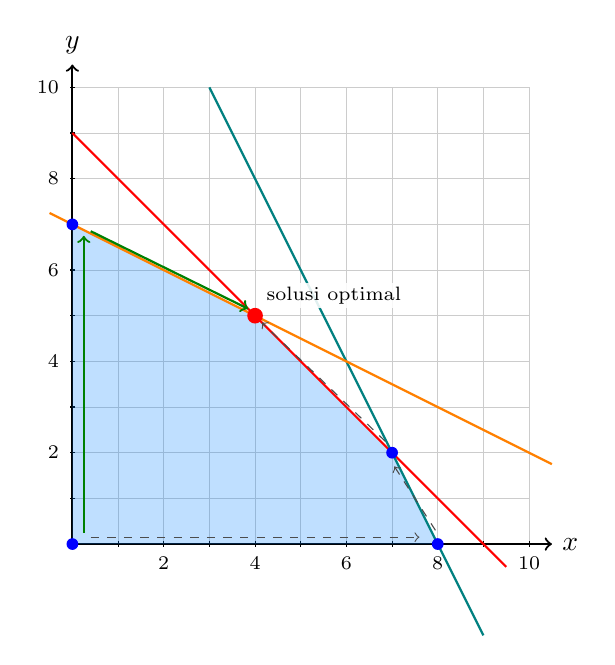
\begin{tikzpicture}[scale=0.58]
    % Grid and axes
    \draw[gray!40, very thin, step=1] (0,0) grid (10,10);
    \draw[->, thick] (0,0) -- (10.5,0) node[right] {$x$};
    \draw[->, thick] (0,0) -- (0,10.5) node[above] {$y$};
    \foreach \x in {1,...,10} \draw (\x,0.06) -- (\x,-0.06);
    \foreach \y in {1,...,10} \draw (0.06,\y) -- (-0.06,\y);
    \foreach \x in {2,4,6,8,10} \node[below] at (\x,-0.08) {\scriptsize \x};
    \foreach \y in {2,4,6,8,10} \node[left] at (-0.08,\y) {\scriptsize \y};

    % Feasible region and constraint boundaries.  Their equations are moved
    % into the adjacent legend so the geometry remains unobstructed.
    \fill[blue!50!cyan, opacity=0.25]
        (0,0) -- (8,0) -- (7,2) -- (4,5) -- (0,7) -- cycle;
    \draw[red,    thick] (0,9)       -- (9.5,-0.5);
    \draw[teal,   thick] (3,10)      -- (9,-2);
    \draw[orange, thick] (-0.5,7.25) -- (10.5,1.75);

    % Vertices.  Coordinates, bases, and objective values are listed in the
    % adjacent table rather than stacked across the graph.
    \node[fill=blue,circle,inner sep=1.5pt] at (0,0) {};
    \node[fill=blue,circle,inner sep=1.5pt] at (8,0) {};
    \node[fill=blue,circle,inner sep=1.5pt] at (7,2) {};
    \node[fill=red, circle,inner sep=2pt]   at (4,5) {};
    \node[fill=blue,circle,inner sep=1.5pt] at (0,7) {};
    \node[anchor=south west, fill=white, fill opacity=0.88,
          text opacity=1, inner sep=1.5pt] at (4.15,5.15)
          {\scriptsize solusi optimal};

    % Pivot arrows along edges (one possible path: (0,0)->(0,7)->(4,5),
    % an alternate path: (0,0)->(8,0)->(7,2)->(4,5)).
    \draw[->, thick, green!50!black] (0.25,0.25)  -- (0.25,6.75);
    \draw[->, thick, green!50!black] (0.4,6.85)   -- (3.85,5.15);
    \draw[->, dashed, gray!60!black] (0.4,0.15)   -- (7.6,0.15);
    \draw[->, dashed, gray!60!black] (7.95,0.3)   -- (7.05,1.7);
    \draw[->, dashed, gray!60!black] (6.85,2.25)  -- (4.15,4.85);
\end{tikzpicture}
\end{minipage}\hfill
\begin{minipage}[c]{0.40\linewidth}
\centering\scriptsize
\textbf{Kendala}\par\smallskip
\begin{tabular}{@{}l@{}}
  \textcolor{red}{$x+y=9$}\\
  \textcolor{teal}{$2x+y=16$}\\
  \textcolor{orange!85!black}{$x+2y=14$}
\end{tabular}

\medskip
\textbf{Titik sudut, basis, dan nilai objektif}\par\smallskip
\renewcommand{\arraystretch}{1.16}%
\begin{tabular}{@{}ccl@{}}
  \textbf{Titik} & \textbf{$B$} & \textbf{$z$}\\ \hline
  $(0,0)$ & $\{s_1,s_2,s_3\}$ & $0$\\
  $(8,0)$ & $\{x,s_1,s_3\}$   & $16$\\
  $(7,2)$ & $\{x,y,s_3\}$     & $20$\\
  $(4,5)$ & $\{x,y,s_2\}$     & $23^{\ast}$\\
  $(0,7)$ & $\{y,s_1,s_2\}$   & $21$
\end{tabular}

\smallskip
$^{\ast}$solusi optimal
\end{minipage}
\par\captionof{figure}{Daerah layak dengan basis dan nilai fungsi objektif pada setiap titik sudut; panah menunjukkan dua lintasan pivot yang menuju titik optimal $(4,5)$.}\label{fig:simplex-basis-driven-tikz08}% fig-num-auto

\end{center}

\begin{remark}{Biaya Tereduksi}\label{def:reduced-cost}
Koefisien variabel nonbasis pada baris objektif adalah \emph{biaya tereduksi} variabel tersebut:
\[
\text{Biaya tereduksi } s_1 = -1, \quad \text{biaya tereduksi } s_3 = -1.
\]

\[
\begin{aligned}
\max \quad 
& z = 23~ \text{\colorbox{purple!20!white}{$- s_1 - s_3$}} \tikzmark{zend2} \\
\st \quad 
& \tikzmark{x2} x = 4 ~ - 2s_1 + s_3, \\
& \tikzmark{y2} y = 5 ~ + s_1 - s_3, \\
& \tikzmark{s22} s_2 = 3~ + 3s_1 - s_3, \\
& x, y, s_1, s_2, s_3 \ge 0.
\end{aligned}
\]

% Panah overlay TikZ (lintasan dikomentari — hapus tanda komentar ketika siap)
%\begin{tikzpicture}[remember picture, overlay, >=stealth]
%%% Red arrows: Non-basic variables
%\draw[->, thick, red]
%  ($(pic cs:zend2)+(0.2,0.3)$) -- ++(1.2,0.1) node[right, red] {Non-basic: $s_1 = 0$};
%\draw[->, thick, red]
%  ($(pic cs:zend2)+(0.4,0.1)$) -- ++(1.5,-0.5) node[right, red] {Non-basic: $s_3 = 0$};
%\end{tikzpicture}

\bigskip

\begin{itemize}
    \item Nilai-nilai ini menunjukkan seberapa besar fungsi objektif \( z \) akan berubah untuk setiap kenaikan satu satuan pada variabel yang bersesuaian, dengan asumsi semua variabel lain dipertahankan tetap dan kelayakan dijaga.
    \item Karena ini adalah masalah maksimisasi, biaya tereduksi \emph{negatif} mengimplikasikan bahwa meningkatkan variabel akan \emph{menurunkan} fungsi objektif.
\end{itemize}

\medskip

\noindent\textbf{Kondisi Optimalitas:}  
Suatu solusi basis layak optimal jika dan hanya jika semua biaya tereduksi variabel nonbasis memenuhi:
\[
\text{(untuk maksimisasi):} \quad \text{biaya tereduksi} \le 0.
\]

\medskip

Dalam kamus ini, biaya tereduksi \(s_1\) dan \(s_3\) keduanya negatif.
Karena itu, tidak ada variabel nonbasis yang dapat masuk untuk meningkatkan \(z\).

\textbf{Oleh karena itu, solusi saat ini optimal.}
\end{remark}

\begin{definition}{Biaya Tereduksi dalam Kamus Sembarang}\label{def:reduced-cost-general}

Misalkan suatu program linier berbentuk standar diberikan oleh
\[
\max \quad \mathbf{c}^\top \mathbf{x} \quad \st \quad A\mathbf{x} = \mathbf{b}, \quad \mathbf{x} \geq 0,
\]
dan misalkan \( B \subseteq \{1, \dots, n\} \) adalah basis dari kolom-kolom \( A \) yang saling bebas linier. \emph{Kamus} yang bersesuaian menyatakan variabel basis dan variabel objektif terhadap variabel nonbasis \( N = \{1, \dots, n\} \setminus B \):

\[
\begin{aligned}
z &= z_0 + \sum_{j \in N} \bar{c}_j x_j \\
x_i &= \bar{b}_i + \sum_{j \in N} \bar{a}_{ij} x_j \quad \text{untuk } i \in B
\end{aligned}
\]

Di sini:
\begin{itemize}
    \item \( x_i \) adalah variabel basis,
    \item \( x_j \) untuk \( j \in N \) adalah variabel nonbasis,
    \item \( z_0 \) adalah nilai fungsi objektif saat ini,
    \item \( \bar{c}_j \) adalah \emph{biaya tereduksi} variabel \( x_j \), dan
    \item \( \bar{b}_i \) adalah nilai variabel basis \( x_i \) ketika \( x_j = 0 \) untuk semua \( j \in N \).
\end{itemize}
\end{definition}

\section{Tidak Ada Basis Awal yang Layak dan Metode Big-M}
\label{sec:big-m-dictionary}

\begin{tryit}
\vizlink{two-phase-simplex}{Simpleks Dua Fase}: saksikan variabel artifisial masuk, Fase 1 mendorongnya keluar, dan peralihan ke Fase 2.
\end{tryit}



\begin{outcome}
\begin{itemize}
\item Menangani kasus ketika basis awal tidak layak
\item Memodifikasi algoritma simpleks menggunakan Metode Big-M untuk menemukan basis awal yang layak
\begin{itemize}
\item Memperkenalkan variabel artifisial pada baris yang melanggar kelayakan awal
\item Menambahkan penalti besar (Big-M) pada variabel artifisial dalam fungsi objektif
\item Menjalankan Simpleks dan melakukan pivot hingga variabel artifisial dapat dihilangkan
\item Menghapus variabel bantu dan melanjutkan algoritma simpleks
\end{itemize}
\end{itemize}
\end{outcome}


Setiap contoh yang dikerjakan sejauh ini dimulai dari titik asal $x=y=0$, tempat variabel slack langsung memberikan solusi basis layak yang jelas. Kemudahan itu hilang begitu masalah memiliki kendala ``$\ge$'': pada titik asal, slack yang bersesuaian bernilai negatif, sehingga kamus awal alaminya \emph{tidak layak} dan tidak ada basis untuk memulai metode simpleks. Bagian ini menunjukkan cara membuat basis awal yang layak menggunakan \emph{variabel artifisial} yang dikenai penalti berupa konstanta besar $M$ (\emph{Metode Big-M}), serta bagaimana perangkat yang sama mengungkapkan bahwa suatu masalah sama sekali tidak memiliki solusi layak.

Perhatikan
\[
\begin{aligned}
\max\quad & 2x + 3y \\
\st\quad & 2x + y \geq 5, \\
& 2x + y \leq 16, \\
& x + 2y \leq 14, \\
& x, y \geq 0.
\end{aligned}
\]
Kendala pertama mengarah ke arah yang tidak sesuai untuk titik awal yang mudah, sehingga titik asal tidak layak dan kita tidak dapat langsung membaca basis awal.

\noindent Secara geometris, titik asal berada di luar daerah layak, sehingga tidak dapat menjadi titik sudut awal:
\begin{center}
% Daerah layak untuk contoh Big-M: maks 2x+3y dengan kendala
% 2x+y>=5, 2x+y<=16, x+2y<=14, x,y>=0.
% Titik sudut (berlawanan arah jarum jam): (5/2,0), (8,0), (6,4), (0,7), (0,5).
% Perhatikan bahwa titik asal berada di luar daerah yang diarsir: 2(0)+0 = 0 < 5.
\begin{minipage}[t]{0.56\linewidth}
\centering
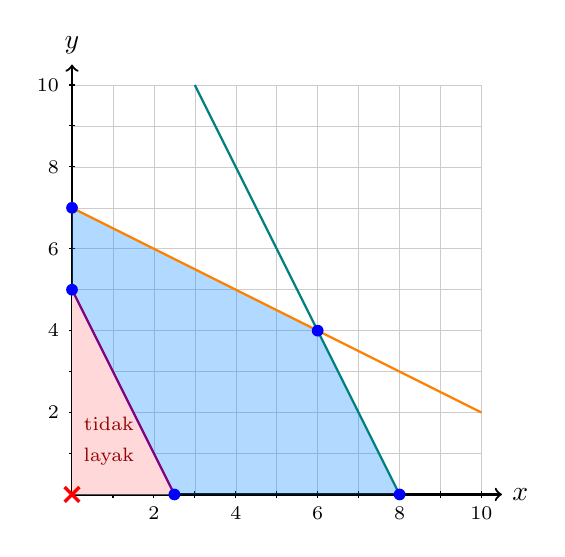
\begin{tikzpicture}[scale=0.52]
    % Grid and axes
    \draw[gray!40, very thin, step=1] (0,0) grid (10,10);
    \draw[->, thick] (0,0) -- (10.5,0) node[right] {$x$};
    \draw[->, thick] (0,0) -- (0,10.5) node[above] {$y$};
    \foreach \x in {1,...,10} \draw (\x,0.08) -- (\x,-0.08);
    \foreach \y in {1,...,10} \draw (0.08,\y) -- (-0.08,\y);
    \foreach \x in {2,4,...,10} \node[below] at (\x,-0.08) {\scriptsize \x};
    \foreach \y in {2,4,...,10} \node[left] at (-0.08,\y) {\scriptsize \y};

    % Shade the infeasible "below 2x+y=5" wedge inside the first quadrant
    % lightly, to emphasize that the origin is cut off.
    \fill[red!15] (0,0) -- (2.5,0) -- (0,5) -- cycle;
    \node[red!60!black, align=center] at (0.9,1.3) {\scriptsize tidak\\[-1pt]\scriptsize layak};

    % Feasible region
    \fill[blue!50!cyan, opacity=0.3]
        (2.5,0) -- (8,0) -- (6,4) -- (0,7) -- (0,5) -- cycle;

    % Constraint boundaries
    % 2x + y = 5 (purple) - the >= constraint
    \draw[violet, thick] (0,5) -- (2.5,0);
    % 2x + y = 16 (teal)
    \draw[teal, thick] (3,10) -- (8,0);
    % x + 2y = 14 (orange)
    \draw[orange, thick] (0,7) -- (10,2);

    % Vertices of feasible region
    \node[fill=blue,circle,inner sep=1.5pt] at (2.5,0) {};
    \node[fill=blue,circle,inner sep=1.5pt] at (8,0)   {};
    \node[fill=blue,circle,inner sep=1.5pt] at (6,4)   {};
    \node[fill=blue,circle,inner sep=1.5pt] at (0,7)   {};
    \node[fill=blue,circle,inner sep=1.5pt] at (0,5)   {};

    % Origin: highlight that it is infeasible (draw a small X)
    \draw[red, very thick] (-0.18,-0.18) -- (0.18,0.18);
    \draw[red, very thick] (-0.18, 0.18) -- (0.18,-0.18);
\end{tikzpicture}
\end{minipage}\hfill
\begin{minipage}[t]{0.40\linewidth}
\small
\textbf{Batas kendala}\par\smallskip
\textcolor{violet}{\(2x+y=5\)} \(\;(\ge)\)\par
\textcolor{teal}{\(2x+y=16\)} \(\;(\le)\)\par
\textcolor{orange}{\(x+2y=14\)} \(\;(\le)\)\par
\medskip
\textbf{Titik sudut daerah layak}\par\smallskip
\(\bigl(\tfrac52,0\bigr),\ (8,0),\ (6,4),\)\par
\((0,7),\ (0,5)\)\par
\medskip
\textcolor{red!70!black}{Tanda \(\times\) merah: titik asal \((0,0)\) tidak layak.}
\end{minipage}

\captionof{figure}{Daerah layak setelah menambahkan kendala \(2x+y\ge 5\): segitiga merah muda di dekat titik asal menjadi tidak layak.}\label{fig:simplex-basis-driven-tikz10}% fig-num-auto

\end{center}


\begin{steppanel}{algslate}
\cstep{1}{Ubah setiap kendala ke bentuk ``$\le$''} Mengalikan kendala $\ge$ dengan $-1$ mengubahnya menjadi kendala $\le$:
\[
\begin{aligned}
\max\quad & 2x + 3y \\
\st\quad & -2x - y \leq -5, \\
& 2x + y \leq 16, \\
& x + 2y \leq 14, \\
& x, y \geq 0.
\end{aligned}
\]
\end{steppanel}

\begin{steppanel}{algslate}
\cstep{2}{Bentuk kamus slack dan temukan ketidaklayakan} Memperkenalkan variabel slack memberikan
\[
\begin{aligned}
\max\quad & 2x + 3y \\
\st\quad & s_1 = -5 + 2x + y,\\
& s_2 = 16 - 2x - y,\\
& s_3 = 14 - x - 2y,\\
& x, y, s_1, s_2, s_3 \ge 0.
\end{aligned}
\]
Pada $x=y=0$, ini memberikan $s_1=-5<0$, sehingga kamus tidak layak dan titik awal simpleks yang biasa tidak tersedia.
\end{steppanel}

\begin{steppanel}{algslate}
\cstep{3}{Perkenalkan variabel artifisial} Tambahkan variabel artifisial nonnegatif $a_1$ ke persamaan yang bermasalah dan kenakan penalti besar pada fungsi objektif (di sini $M=1000$), sehingga metode simpleks terdorong mengembalikannya ke nol:
\[
\begin{aligned}
\max\quad & 2x + 3y - 1000a_1 \\
\st\quad & s_1 = -5 + 2x + y + a_1,\\
& s_2 = 16 - 2x - y,\\
& s_3 = 14 - x - 2y,\\
& x, y, s_1, s_2, s_3, a_1 \ge 0.
\end{aligned}
\]
\end{steppanel}

\begin{steppanel}{algslate}
\cstep{4}{Pivot ke basis layak} Menukar $a_1$ ke dalam basis untuk menggantikan $s_1$ membuat setiap ruas kanan nonnegatif pada $x=y=0$, sehingga memberikan titik awal yang sah:
\[
\begin{aligned}
\max\quad & -5000 + 2002x + 1003y - 1000s_1 \\
\st\quad & a_1 = 5 - 2x - y + s_1,\\
& s_2 = 16 - 2x - y,\\
& s_3 = 14 - x - 2y,\\
& x, y, s_1, s_2, s_3, a_1 \ge 0.
\end{aligned}
\]
\end{steppanel}

Dengan basis layak yang telah diperoleh, kita menjalankan metode simpleks seperti biasa. Membiarkan $x$ masuk mendorong variabel artifisial kembali keluar dari basis:
\[
\begin{aligned}
\max\quad & 5 + 2y + s_1 - 1001a_1 \\
\st\quad & x = 2.50 - 0.50y + 0.50s_1 - 0.50a_1,\\
& s_2 = 11 - s_1 + a_1,\\
& s_3 = 11.50 - 1.50y - 0.50s_1 + 0.50a_1,\\
& x, y, s_1, s_2, s_3, a_1 \ge 0.
\end{aligned}
\]

\noindent Struktur kamus layak ini layak dicermati sejenak.
\begin{remark}{Variabel Artifisial Dapat Dihilangkan: Titik Awal Layak untuk Fase II}{}
Ini adalah kamus artifisial kedua dari \textbf{Fase I} metode simpleks dua fase. Tujuan kita adalah mengeliminasi variabel artifisial \(a_1\) sambil menemukan solusi layak bagi masalah semula.

Perhatikan kamus ini:
\begin{itemize}
    \item Variabel artifisial \(a_1\) muncul dalam sistem, tetapi \textbf{bukan variabel basis}.
    \item Karena \(a_1\) merupakan variabel nonbasis dan nilainya saat ini nol, variabel tersebut dapat \textbf{dihilangkan} dari kamus tanpa melanggar kelayakan.
    \item Semua variabel basis (\(x, s_2, s_3\)) memiliki nilai nonnegatif ketika \(a_1 = 0\), dan semua koefisien \(a_1\) dapat langsung dihapus.
\end{itemize}

\textbf{Kesimpulan:} Sekarang kita memiliki solusi basis layak bagi masalah semula (tanpa variabel artifisial), sehingga kita dapat memulai \textbf{Fase II metode simpleks} menggunakan kamus ini sebagai titik awal.

\vspace{1cm}

\[
\begin{aligned}
\max \quad 
& \tikzmark{zstart4} \text{\colorbox{green!20!white}{$5$}} ~ \text{\colorbox{gray!20!white}{$+ 2y + s_1 - 1001a_1$}} \tikzmark{zend4} \\
\st \quad 
& \tikzmark{xx4} \text{\colorbox{yellow}{$x = 2.50$}} ~ \text{\colorbox{gray!20!white}{$- 0.50y + 0.50s_1 - 0.50a_1$}},\\[1mm]
& \tikzmark{s24} \text{\colorbox{yellow}{$s_2 = 11$}} ~ \text{\colorbox{gray!20!white}{$- s_1 + a_1$}},\\[1mm]
& \tikzmark{s34} \text{\colorbox{yellow}{$s_3 = 11.50$}} ~ \text{\colorbox{gray!20!white}{$- 1.50y - 0.50s_1 + 0.50a_1$}},\\[1mm]
& x,\, y,\, s_1,\, s_2,\, s_3,\, a_1 \ge 0.
\end{aligned}
\]

\begin{tikzpicture}[remember picture, overlay, >=stealth]

% Arrows: basic variables
\draw[->, thick, blue] 
  ($(pic cs:xx4)+(-0.2,-0.2)$) -- ++(-3.0,-0.5) node[left, blue] {Variabel basis: $x = 2.50$};
\draw[->, thick, blue] 
  ($(pic cs:s24)+(-0.2,-0.2)$) -- ++(-3.0,-0.5) node[left, blue] {Variabel basis: $s_2 = 11$};
\draw[->, thick, blue] 
  ($(pic cs:s34)+(-0.2,-0.2)$) -- ++(-3.0,-0.5) node[left, blue] {Variabel basis: $s_3 = 11.50$};

% Red arrow: nonbasic artificial variable
\draw[->, thick, red] 
  ($(pic cs:zend4)+(0.4,0.3)$) -- ++(2,0.5) node[right, red] {Nonbasis: $a_1 = 0$};

\end{tikzpicture}
\end{remark}

\begin{learningcheckpoint}[label={lc:artificial-removal}]
Mengapa variabel artifisial dapat dihilangkan dari sistem ini?
\end{learningcheckpoint}

Sekarang $a_1$ adalah variabel nonbasis, sehingga basis layak bagi masalah \emph{semula}. Kita dapat membuang variabel artifisial dan melanjutkan dari kamus layak
\[
\begin{aligned}
\max\quad & 5 + 2y + s_1 \\
\st\quad & x = 2.50 - 0.50y + 0.50s_1,\\
& s_2 = 11 - s_1,\\
& s_3 = 11.50 - 1.50y - 0.50s_1,\\
& x, y, s_1, s_2, s_3 \ge 0.
\end{aligned}
\]

\subsection{Algoritma Metode Big-M}

\begin{algocard}{Algoritma: Metode Big-M}
\textbf{Masukan.} Suatu program linier berbentuk standar (maksimisasi), mungkin dengan solusi basis awal yang tidak layak.
\algostep{algenter}{\ding{43}}{Tambahkan variabel artifisial}{Untuk setiap kendala dengan ruas kanan negatif, kalikan kendala dengan $-1$ agar ruas kanan menjadi positif. Untuk setiap kendala tanpa variabel basis layak yang jelas, tambahkan variabel artifisial $a_i \ge 0$.}
\algostep{algleave}{\ding{47}}{Kenakan penalti pada variabel artifisial}{Tambahkan suku penalti $-M a_i$ (dengan $M$ konstanta yang sangat besar) untuk setiap variabel artifisial ke fungsi objektif. Bentuk kamus awal (termasuk variabel slack/surplus dan artifisial) menggunakan fungsi objektif yang dimodifikasi ini, dengan variabel artifisial berada dalam basis awal.}
\algostep{algpivot}{\ding{114}}{Dorong variabel artifisial keluar}{Selama suatu variabel artifisial berada dalam basis (atau solusi basis tidak layak), lakukan pivot simpleks menggunakan fungsi objektif yang dimodifikasi, yang memindahkan setidaknya satu variabel artifisial keluar dari basis.}
\algostep{algenter}{\ding{43}}{Pulihkan dan lanjutkan}{Setelah semua variabel artifisial bernilai nol, hapus kolom-kolomnya dan lanjutkan iterasi simpleks standar menggunakan fungsi objektif \emph{semula}.}
\algostep{algopt}{\ding{52}}{Keluaran}{Solusi optimal bagi masalah semula, atau pernyataan ketidaklayakan jika ada variabel artifisial yang tetap positif.}
\end{algocard}

%
%
\subsection{Mendeteksi Ketidaklayakan melalui Metode Big-M}

Perhatikan program linier
\[
\begin{aligned}
\max\quad & 2x + 3y \\
\st\quad & 2x + y \geq 22,\quad 2x + y \leq 16,\quad x + 2y \leq 14,\quad x,y \geq 0.
\end{aligned}
\]
Dua kendala pertama menuntut agar $2x+y$ secara bersamaan sedikitnya $22$ dan paling banyak $16$, sehingga kita patut memperkirakan adanya masalah. Menulis ulang kendala $\ge$ sebagai $-2x-y\le-22$ dan menambahkan slack memberikan $s_1 = -22 + 2x + y$, yang negatif pada titik asal. Sama persis seperti sebelumnya, kita menambahkan variabel artifisial $a_1$ (penalti $M=1000$) dan melakukan pivot untuk memasukkannya ke basis guna memperoleh kamus awal yang layak:
\begin{center}\begin{dict}
\[
\begin{aligned}
\max\quad & -22000 + 2002x + 1003y - 1000s_1 \\
\st\quad & a_1 = 22 - 2x - y + s_1,\\
& s_2 = 16 - 2x - y,\\
& s_3 = 14 - x - 2y.
\end{aligned}
\]
\end{dict}\end{center}
\pivotstrip{x}{s_2}{}
\begin{center}\begin{dict}
\[
\begin{aligned}
\max\quad & -5984 + 2y - 1000s_1 - 1001s_2 \\
\st\quad & a_1 = 6 + s_1 + s_2,\\
& x = 8 - 0.50y - 0.50s_2,\\
& s_3 = 6 - 1.50y + 0.50s_2.
\end{aligned}
\]
\end{dict}\end{center}
\pivotstrip{y}{s_3}{}
\begin{center}
\begin{tcolorbox}[enhanced,width=0.6\linewidth,box align=center,colback=red!4,colframe=red!65!black,
  boxrule=0.8pt,sharp corners,coltitle=white,fonttitle=\bfseries,
  title={\ding{56}\ Optimal untuk Big-M: variabel artifisial tersangkut dalam basis},
  left=6pt,right=6pt,top=3pt,bottom=3pt]
\[
\begin{aligned}
\max\quad & -5976 - 1000s_1 - 1000.33s_2 - 1.33s_3 \\
\st\quad & a_1 = 6 + s_1 + s_2,\\
& x = 6 - 0.67s_2 + 0.33s_3,\\
& y = 4 + 0.33s_2 - 0.67s_3.
\end{aligned}
\]
\end{tcolorbox}
\end{center}
Setiap koefisien baris objektif sekarang nonpositif, sehingga kamus ini optimal untuk masalah berpenalti (Big-M), tetapi variabel artifisial masih merupakan variabel basis.

\subsection*{Menafsirkan Kamus Akhir}

Dalam kamus akhir, variabel artifisial \(a_1\) muncul dalam persamaan
\[
a_1 = 6 + s_1 + s_2.
\]
Ketika variabel nonbasis \(s_1\) dan \(s_2\) ditetapkan sama dengan nol (seperti yang lazim dalam suatu solusi basis), kita memperoleh
\[
a_1 = 6.
\]
Karena \(a_1 > 0\) dalam kamus optimal, hal ini menunjukkan bahwa program linier semula tidak memiliki solusi layak. Kehadiran variabel artifisial positif dalam kamus optimal akhir merupakan sinyal standar dalam Metode Big-M bahwa masalah semula tidak layak.

\bigskip

\noindent Ringkasnya, kendala yang saling bertentangan (yang mengharuskan \(2x+y\) sekaligus sedikitnya 22 dan paling banyak 16) memaksa variabel artifisial \(a_1\) tetap positif. Dengan demikian, Metode Big-M menegaskan bahwa masalah tersebut tidak layak.

\begin{remark}{Kamus Artifisial Akhir Menunjukkan Ketidaklayakan}{}
Ini adalah kamus akhir pada akhir \textbf{Fase I} metode simpleks dua fase, yang tujuannya mengeliminasi variabel artifisial \(a_1\) dan mencapai solusi layak bagi masalah semula.

Untuk menafsirkannya:
\begin{itemize}
    \item Variabel artifisial \(a_1\) masih berada dalam basis.
    \item Nilainya dinyatakan sebagai \(a_1 = 6 + s_1 + s_2\), dan karena semua variabel di ruas kanan dibatasi agar nonnegatif, kita memiliki \(a_1 \ge 6\).
    \item Oleh karena itu, kita tidak dapat membuat \(a_1 = 0\), yang diperlukan untuk mencapai kelayakan pada Fase I.
\end{itemize}

Jadi, tidak ada solusi layak bagi masalah semula.  \\
\textbf{Kesimpulan: Program linier semula \emph{tidak layak}.}

\vspace{1cm}

\[
\begin{aligned}
\max \quad 
& \tikzmark{zstart3} \text{\colorbox{green!20!white}{$-5976$}} ~ \text{\colorbox{red!50!white}{$- 1000s_1 - 1000.33s_2 - 1.33s_3$}} \tikzmark{zend3} \\
\st \quad 
& \tikzmark{a1} \text{\colorbox{red!50!white}{$a_1 = 6$}} ~ \text{\colorbox{gray!20!white}{$+ s_1 + s_2$}},\\[1mm]
& \tikzmark{x3} \text{\colorbox{yellow}{$x = 6$}} ~ \text{\colorbox{gray!20!white}{$- 0.67s_2 + 0.33s_3$}},\\[1mm]
& \tikzmark{y3} \text{\colorbox{yellow}{$y = 4$}} ~ \text{\colorbox{gray!20!white}{$+ 0.33s_2 - 0.67s_3$}},\\[1mm]
& x, y, s_1, s_2, s_3, a_1 \geq 0.
\end{aligned}
\]

\begin{tikzpicture}[remember picture, overlay, >=stealth]

% Blue arrows: Basic variables
\draw[->, thick, red] 
  ($(pic cs:a1)+(-0.2,-0.2)$) -- ++(-3.0,-0.5) node[left, red] {$a_1$ masih berada dalam basis};
%\draw[->, thick, blue]
%  ($(pic cs:x3)+(-0.2,-0.2)$) -- ++(-3.0,-0.5) node[left, blue] {Basic var: $x = 6$};
%\draw[->, thick, blue]
%  ($(pic cs:y3)+(-0.2,-0.2)$) -- ++(-3.0,-0.5) node[left, blue] {Basic var: $y = 4 $};

% Red arrows: Nonbasic variables s_1, s_2, s_3
\draw[->, thick, red] 
  ($(pic cs:zend3)+(-2.3,0.4)$) -- ++(0.8,0.5) node[right, red] {Semua koefisien objektif $\leq 0$};

\end{tikzpicture}
\end{remark}

\begin{theorem}{Deteksi Ketidaklayakan melalui Metode Big-M}{}
Perhatikan masalah program linier
\[
\begin{aligned}
\max\quad & \mathbf{c}^\top \mathbf{x} \\
\st\quad & A\mathbf{x} \le \mathbf{b}, \\
& \mathbf{x} \ge \mathbf{0}.
\end{aligned}
\]
Setelah mengonversi pertidaksamaan menjadi persamaan dengan memperkenalkan variabel slack, surplus, dan, jika diperlukan, artifisial, sistem berbentuk
\[
A\mathbf{x} - I_a \mathbf{a} = \mathbf{b},\quad \mathbf{x},\, \mathbf{a} \ge \mathbf{0},
\]
dengan \( I_a \) adalah submatriks dari matriks identitas, yang setiap kolomnya berkorespondensi dengan variabel artifisial yang diperkenalkan untuk memberlakukan persamaan pada kendala yang semula tidak memiliki variabel basis dengan ruas kanan nonnegatif. Perumusan Big-M kemudian diberikan oleh
\[
\max\quad \mathbf{c}^\top \mathbf{x} - M\sum_{i\in I} a_i.
\]
Jika, dalam sembarang solusi optimal masalah Big-M, terdapat variabel artifisial \(a_i > 0\) untuk suatu \(i\in I\), maka masalah program linier semula tidak layak.
\end{theorem}

\begin{proof}
Asumsikan bahwa solusi optimal \((\mathbf{x}^*,\mathbf{a}^*)\) dari masalah Big-M memenuhi \(a_i^* > 0\) untuk suatu \(i\in I\).

Andaikan, demi kontradiksi, masalah program linier semula layak. Maka terdapat suatu \(\mathbf{x}'\ge \mathbf{0}\) sedemikian sehingga \(A\mathbf{x}' \le \mathbf{b}\). Dalam proses perumusan ulang, jika suatu kendala tidak memiliki variabel basis dengan ruas kanan nonnegatif, variabel artifisial \(a_i\) diperkenalkan dengan menulis ulang kendala sebagai
\[
\text{(kendala semula)} - a_i = b_i.
\]
Untuk sembarang \(\mathbf{x}'\) yang layak bagi masalah semula, kita dapat menetapkan \(\mathbf{a}' = \mathbf{0}\) untuk semua variabel artifisial, dan kendala persamaan tetap akan terpenuhi.

Dengan demikian, solusi \((\mathbf{x}',\mathbf{0})\) layak bagi perumusan Big-M, dan nilai fungsi objektifnya tepat \(\mathbf{c}^\top \mathbf{x}'\). Di sisi lain, solusi optimal \((\mathbf{x}^*,\mathbf{a}^*)\) menghasilkan nilai fungsi objektif 
\[
\mathbf{c}^\top \mathbf{x}^* - M\sum_{i\in I}a_i^*.
\]
Karena \(M\) dipilih sebagai konstanta positif yang sangat besar, setiap kontribusi positif dari \(\sum_{i\in I}a_i^*\) memberikan penalti berat. Akibatnya, nilai fungsi objektif \((\mathbf{x}',\mathbf{0})\) akan lebih besar secara tegas daripada nilai fungsi objektif \((\mathbf{x}^*,\mathbf{a}^*)\), asalkan \(M\) cukup besar.

Kontradiksi ini mengimplikasikan bahwa tidak ada solusi layak \((\mathbf{x}',\mathbf{0})\) bagi masalah semula. Dengan kata lain, asumsi bahwa masalah semula layak adalah salah.

Jadi, jika dalam solusi optimal masalah Big-M ada variabel artifisial yang tetap positif, masalah program linier semula pasti tidak layak.
\end{proof}

\subsection{Contoh kedua: dua variabel artifisial}

Ketika beberapa kendala mengarah ke arah yang ``salah'', kita cukup menambahkan satu variabel artifisial untuk setiap kendala yang bermasalah. Perhatikan
\[
\begin{aligned}
\max\quad & 3x + y \\
\st\quad & 2x + y \geq 5,\quad 2x + y \leq 16,\quad x + 2y \geq 3,\quad x,y \geq 0.
\end{aligned}
\]
Dua kendala bertipe ``$\ge$'', sehingga titik asal melanggar keduanya. Membaliknya menjadi $-2x-y\le-5$ dan $-x-2y\le-3$ serta menambahkan slack memberikan $s_1 = -5 + 2x + y$ dan $s_3 = -3 + x + 2y$, yang keduanya negatif pada titik asal. Kita memperkenalkan \emph{dua} variabel artifisial $a_1,a_3$ (masing-masing dikenai penalti $M=1000$) dan melakukan pivot untuk memasukkannya ke basis, sehingga menghasilkan kamus awal layak yang baris objektifnya memuat penalti Big-M:
\begin{center}\begin{dict}
\[
\begin{aligned}
\max\quad & -8000 + 3003x + 3001y \\
           & \qquad {}- 1000s_1 - 1000s_3 \\
\st\quad & a_1 = 5 - 2x - y + s_1,\\
& s_2 = 16 - 2x - y,\\
& a_3 = 3 - x - 2y + s_3.
\end{aligned}
\]
\end{dict}\end{center}
Penalti yang besar membuat peningkatan $x$ dan $y$ menarik, dan pivot berturut-turut mendorong kedua variabel artifisial keluar dari basis. Setelah $a_1=a_3=0$, basis layak bagi masalah semula; kita menghapus variabel artifisial dan melanjutkan pada fungsi objektif sebenarnya $3x+y$ sampai setiap biaya tereduksi nonpositif:
\begin{center}\begin{dictopt}
\[
\begin{aligned}
\max\quad & 24 - 0.5\,y - 1.5\,s_2 \\
\st\quad & x = 8 - 0.5\,y - 0.5\,s_2,\\
& s_1 = 11 - s_2,\\
& s_3 = 5 + 1.5\,y - 0.5\,s_2.
\end{aligned}
\]
\end{dictopt}\end{center}
Membaca kamus optimal memberikan $x = 8$, $y = 0$, dan $z = 3x + y = 24$, dengan kendala pertama dan ketiga memiliki slack ($s_1=11$, $s_3=5$) dan kendala kedua ketat ($s_2=0$).

\section{Degenerasi, Siklus, dan Aturan Bland}
\label{sec:degeneracy}

\begin{definition}{Degenerasi}{}
Suatu solusi basis layak (BFS) dalam Metode Simpleks disebut \textbf{degenerat} jika satu atau lebih variabel basisnya bernilai nol. Secara matematis, BFS yang berkorespondensi dengan suatu basis \( B \) bersifat degenerat jika terdapat setidaknya satu variabel basis \( \x_B \) sedemikian sehingga \( \x_B = 0 \).
\end{definition}

\begin{remark}{Kamus Degenerat}{}
Kamus di bawah ini merepresentasikan solusi layak, tetapi salah satu variabel basis sama dengan nol. Situasi ini disebut \textbf{degenerasi}.

\textbf{Apa itu degenerasi?}  
Suatu kamus disebut \emph{degenerat} jika \textbf{ada variabel basis yang sama dengan nol}. Hal ini penting karena:
\begin{itemize}
    \item Ini dapat menyebabkan metode simpleks melakukan pivot tanpa mengubah nilai fungsi objektif.
    \item Ini berpotensi menyebabkan \textbf{siklus}, yaitu mengunjungi kembali solusi basis yang sama lebih dari sekali.
\end{itemize}

\textbf{Dalam kamus ini:}
\begin{itemize}
    \item Variabel basis adalah \(x_3, x_4, x_5, x_6\).
    \item Ketika kita menetapkan variabel nonbasis \(x_1 = 0\), \(x_2 = 0\), kita memperoleh:
    \[
    x_3 = 4,\quad x_4 = 2,\quad x_5 = 3,\quad x_6 = \boxed{0},\quad z = 0.
    \]
    \item Karena \(x_6 = 0\) dan berada dalam basis, ini adalah \textbf{solusi basis layak degenerat}.
\end{itemize}

\vspace{1cm}

\[
\begin{aligned}
\max \quad 
& \tikzmark{zstart5} \text{\colorbox{green!20!white}{$z = 0$}} ~ \text{\colorbox{gray!20!white}{$+ x_1 + 2x_2$}} \tikzmark{zend5} \\
\st \quad 
& \tikzmark{x3} \text{\colorbox{yellow}{$x_3 = 4$}} ~ \text{\colorbox{gray!20!white}{$- x_2$}}, \\
& \tikzmark{x4} \text{\colorbox{yellow}{$x_4 = 2$}} ~ \text{\colorbox{gray!20!white}{$- x_1 + x_2$}}, \\
& \tikzmark{x5} \text{\colorbox{yellow}{$x_5 = 3$}} ~ \text{\colorbox{gray!20!white}{$- x_1$}}, \\
& \tikzmark{x6} \text{\colorbox{orange}{$x_6 = 0$}} ~ \text{\colorbox{gray!20!white}{$+ 2x_1 - x_2$}}, \\
& x_1, x_2, x_3, x_4, x_5, x_6 \geq 0.
\end{aligned}
\]

\begin{tikzpicture}[remember picture, overlay, >=stealth]

% Arrows to show basic variables and highlight degeneracy
\draw[->, thick, blue] 
  ($(pic cs:x3)+(-0.2,-0.2)$) -- ++(-3.0,-0.5) node[left, blue] {Variabel basis: $x_3 = 4$};
\draw[->, thick, blue] 
  ($(pic cs:x4)+(-0.2,-0.2)$) -- ++(-3.0,-0.5) node[left, blue] {Variabel basis: $x_4 = 2$};
\draw[->, thick, blue] 
  ($(pic cs:x5)+(-0.2,-0.2)$) -- ++(-3.0,-0.5) node[left, blue] {Variabel basis: $x_5 = 3$};
\draw[->, thick, orange, ultra thick] 
  ($(pic cs:x6)+(-0.2,-0.2)$) -- ++(-3.0,-0.5) node[left, orange] {\textbf{Degenerat: $x_6 = 0$}};

% Optional: arrows to nonbasic variables
\draw[->, thick, red!60!black] 
  ($(pic cs:zend5)+(0.3,0.1)$) -- ++(1.5,0.6) node[right, red!60!black] {Nonbasis: $x_1 = x_2 = 0$};

\end{tikzpicture}
\end{remark}

Dalam kasus ini, solusi basis layaknya adalah (variabel basis) $(x_3,x_4, x_5,x_6) = (4,2,3,0)$ dan (variabel nonbasis) $(x_1, x_2) = (0,0)$.

\subsection{Degenerasi dan BFS yang Tidak Berubah setelah Pivot}
Degenerasi dapat menimbulkan kasus ketika pivot dalam Metode Simpleks tidak mengubah solusi basis layak. Ketika pivot dilakukan, variabel masuk ditingkatkan sampai salah satu variabel basis saat ini mencapai nol, dan pada saat itu variabel tersebut keluar dari basis. Namun, jika beberapa kendala menghasilkan rasio minimum yang sama pada uji rasio, maka aturan pemecah hasil imbang harus diterapkan. Jika variabel yang keluar dari basis sudah bernilai nol, BFS tetap tidak berubah. 

Perhatikan bahwa dalam contoh sebelumnya, kita dapat mencoba membiarkan $x_2$ masuk ke basis. Apa yang terjadi? Berdasarkan uji rasio, kita melihat bahwa $x_6$ keluar dari basis. Ini menghasilkan kamus baru berikut:

\begin{remark}{Pivot Degenerat: BFS Tidak Berubah}{}
Setelah melakukan pivot untuk memasukkan \(x_2\) ke basis dan mengeluarkan \(x_6\), kita memperoleh kamus di bawah ini. 

Inilah yang terjadi:

\begin{itemize}
    \item Sebelum pivot, variabel basis adalah \(x_3, x_4, x_5, x_6\), dan variabel nonbasis adalah \(x_1 = 0, x_2 = 0\).
    \item Setelah pivot, \(x_2\) masuk dan \(x_6\) keluar. Variabel basis baru adalah \(x_3, x_4, x_5, x_2\).
    \item Namun, ketika kita memasukkan nilai nonbasis \(x_1 = 0, x_6 = 0\), kita memperoleh:
    \[
    x_3 = 4, \quad x_4 = 2, \quad x_5 = 3, \quad x_2 = 0, \quad z = 0.
    \]
    \item Ini \textbf{identik dengan solusi basis layak sebelumnya}.
\end{itemize}

\textbf{Kesimpulan:}  
Ini adalah kasus \textbf{pivot degenerat}: kita melakukan langkah pivot, tetapi solusi basis layak yang dihasilkan tidak berubah. Algoritma simpleks berpindah ke kamus baru (yaitu, basis baru), tetapi titik dalam ruang solusi tetap sama.

\vspace{1cm}

\[
\begin{aligned}
\max \quad 
& \tikzmark{zstart6} \text{\colorbox{green!20!white}{$z = 0$}} ~ \text{\colorbox{gray!20!white}{$+ 5x_1 - 2x_6$}} \tikzmark{zend6} \\
\st \quad 
& \tikzmark{x3b} \text{\colorbox{yellow}{$x_3 = 4$}} ~ \text{\colorbox{gray!20!white}{$- 2x_1 + x_6$}},\\ 
& \tikzmark{x4b} \text{\colorbox{yellow}{$x_4 = 2$}} ~ \text{\colorbox{gray!20!white}{$+ x_1 - x_6$}},\\ 
& \tikzmark{x5b} \text{\colorbox{yellow}{$x_5 = 3$}} ~ \text{\colorbox{gray!20!white}{$- x_1$}},\\ 
& \tikzmark{x2b} \text{\colorbox{orange}{$x_2 = 0$}} ~ \text{\colorbox{gray!20!white}{$+ 2x_1 - x_6$}},\\
& x_1, x_2, x_3, x_4, x_5, x_6 \ge 0.
\end{aligned}
\]

\begin{tikzpicture}[remember picture, overlay, >=stealth]

% Blue: basic variables
\draw[->, thick, blue] 
  ($(pic cs:x3b)+(-0.2,-0.2)$) -- ++(-3.0,-0.5) node[left, blue] {Variabel basis: $x_3 = 4$};
\draw[->, thick, blue] 
  ($(pic cs:x4b)+(-0.2,-0.2)$) -- ++(-3.0,-0.5) node[left, blue] {Variabel basis: $x_4 = 2$};
\draw[->, thick, blue] 
  ($(pic cs:x5b)+(-0.2,-0.2)$) -- ++(-3.0,-0.5) node[left, blue] {Variabel basis: $x_5 = 3$};
\draw[->, thick, red] 
  ($(pic cs:x2b)+(-0.2,-0.2)$) -- ++(-3.0,-0.5) node[left, orange] {\textbf{Basis baru: $x_2 = 0$ (degenerat)}};

% Arrow to objective
\draw[->, thick, green!60!black] 
  ($(pic cs:zstart6)+(0,0.2)$) -- ++(-2.5,1.0) node[left, green!60!black] {Objektif: $z = 0$};

% Arrow to nonbasic values
\draw[->, thick, red!60!black] 
  ($(pic cs:zend6)+(0.3,0.1)$) -- ++(1.8,0.6) node[right, red!60!black] {Nonbasis: $x_1 = 0$, $x_6 = 0$};

\end{tikzpicture}
\end{remark}

Namun! Solusi basis layaknya tetap sama!!!

Untungnya, pivot berikutnya menghasilkan solusi baru.

Namun, fenomena ini dapat menyebabkan algoritma mengunjungi BFS yang sama beberapa kali, sehingga berpotensi menimbulkan siklus.

Lihat \url{https://gilp.henryrobbins.com/en/latest/examples/3d/SQUARE_PYRAMID_3D_LP.html} untuk kasus yang sangat degenerat ketika dua pivot pertama tidak mengubah solusi.

\section{Siklus dalam Metode Simpleks}

Dalam Metode Simpleks, operasi pivot biasanya memperbaiki fungsi objektif dengan berpindah dari satu solusi basis layak (BFS) ke solusi lain. Namun, dalam kasus yang jarang terjadi, metode ini dapat mengunjungi kembali \emph{BFS yang sama beberapa kali} tanpa kemajuan. Fenomena ini disebut \textbf{siklus}.

Siklus terjadi karena:
\begin{itemize}
  \item \textbf{Degenerasi}: ketika satu atau lebih variabel basis bernilai nol.
  \item \textbf{Aturan pivot yang kurang beruntung}: yang menyebabkan algoritma berputar melalui basis-basis berbeda yang berkorespondensi dengan BFS yang sama.
\end{itemize}

Contoh berikut menunjukkan siklus. Variabel masuk dipilih berdasarkan \textbf{aturan koefisien terbesar}, dan hasil imbang pada uji rasio minimum diputus secara naif, dengan mengambil baris berimbang yang variabel basisnya dicantumkan pertama. Kombinasi ini mengalami siklus pada contoh di bawah. Aturan pivot antisiklus, seperti aturan leksikografis atau Aturan Bland (yang dijelaskan nanti dalam bagian ini), mencegah perilaku tersebut.

\subsection{Siklus dalam Metode Simpleks}
Siklus terjadi ketika Metode Simpleks berulang kali mengunjungi kembali himpunan variabel basis yang sama tanpa membuat kemajuan dalam memperbaiki fungsi objektif. Ini terjadi ketika ada degenerasi dan pilihan variabel masuk dan keluar menghasilkan perulangan di antara sekumpulan BFS degenerat.

Contoh berikut menunjukkan siklus dalam Metode Simpleks. Contoh ini merupakan versi berskala ulang dari contoh siklus klasik yang dibuat oleh E.~M.~L.~Beale (1955), contoh PL terpublikasi pertama yang membuat metode simpleks mengalami siklus; hanya satuan dua variabel yang diubah, dan hal ini mempertahankan siklus tersebut.

\textbf{Kamus Awal}
\[
\begin{aligned}
\max \quad & z = 0 + 0.75x_1 - 20x_2 + 0.50x_3 - 6x_4 \\
\st \quad 
& s_1 = 0 - 0.25x_1 + 8x_2 + x_3 - 9x_4, \\
& s_2 = 0 - 0.50x_1 + 12x_2 + 0.50x_3 - 3x_4, \\
& s_3 = 1 - x_3, \\
& x_1, x_2, x_3, x_4, s_1, s_2, s_3 \geq 0.
\end{aligned}
\]

\pivotstrip{x_1}{s_1}{}
\[
\begin{aligned}
\max \quad & z = 0 + 4x_2 + 3.50x_3 - 33x_4 - 3s_1 \\
\st \quad 
& x_1 = 0 + 32x_2 + 4x_3 - 36x_4 - 4s_1, \\
& s_2 = 0 - 4x_2 - 1.50x_3 + 15x_4 + 2s_1, \\
& s_3 = 1 - x_3, \\
& x_1, x_2, x_3, x_4, s_1, s_2, s_3 \geq 0.
\end{aligned}
\]

\pivotstrip{x_2}{s_2}{}
\[
\begin{aligned}
\max \quad & z = 0 + 2x_3 - 18x_4 - s_1 - s_2 \\
\st \quad 
& x_1 = 0 - 8x_3 + 84x_4 + 12s_1 - 8s_2, \\
& x_2 = 0 - 0.38x_3 + 3.75x_4 + 0.50s_1 - 0.25s_2, \\
& s_3 = 1 - x_3, \\
& x_1, x_2, x_3, x_4, s_1, s_2, s_3 \geq 0.
\end{aligned}
\]

\pivotstrip{x_3}{x_1}{}
\[
\begin{aligned}
\max \quad & z = 0 - 0.25x_1 + 3x_4 + 2s_1 - 3s_2 \\
\st \quad 
& x_3 = 0 - 0.12x_1 + 10.50x_4 + 1.50s_1 - s_2, \\
& x_2 = 0 + 0.05x_1 - 0.19x_4 - 0.06s_1 + 0.12s_2, \\
& s_3 = 1 + 0.12x_1 - 10.50x_4 - 1.50s_1 + s_2, \\
& x_1, x_2, x_3, x_4, s_1, s_2, s_3 \geq 0.
\end{aligned}
\]
\pivotstrip{x_4}{x_2}{}
\[
\begin{aligned}
\max \quad & z = +0.50x_1 - 16x_2 + s_1 - s_2 \\
\st \quad 
& x_3 = 0 + 2.50x_1 - 56x_2 - 2s_1 + 6s_2, \\
& x_4 = 0 + 0.25x_1 - 5.33x_2 - 0.33s_1 + 0.67s_2, \\
& s_3 = 1 - 2.50x_1 + 56x_2 + 2s_1 - 6s_2, \\
& x_1, x_2, x_3, x_4, s_1, s_2, s_3 \geq 0.
\end{aligned}
\]
\pivotstrip{s_1}{s_3}{}

\[
\begin{aligned}
\max \quad & z = +1.75x_1 - 44x_2 - 0.50x_3 + 2s_2 \\
\st \quad 
& s_1 = 0 + 1.25x_1 - 28x_2 - 0.50x_3 + 3s_2, \\
& x_4 = 0 - 0.17x_1 + 4x_2 + 0.17x_3 - 0.33s_2, \\
& s_3 = 1 - x_3, \\
& x_1, x_2, x_3, x_4, s_1, s_2, s_3 \geq 0.
\end{aligned}
\]
\pivotstrip{s_2}{x_4}{}
\[
\begin{aligned}
\max \quad & z = +0.75x_1 - 20x_2 + 0.50x_3 - 6x_4 \\
\st \quad 
& s_1 = 0 - 0.25x_1 + 8x_2 + x_3 - 9x_4, \\
& s_2 = 0 - 0.50x_1 + 12x_2 + 0.50x_3 - 3x_4, \\
& s_3 = 1 - x_3, \\
& x_1, x_2, x_3, x_4, s_1, s_2, s_3 \geq 0.
\end{aligned}
\]

\noindent Kamus terakhir ini \emph{identik} dengan kamus awal: setelah enam pivot, metode telah kembali ke basis awalnya dengan fungsi objektif tetap pada $z=0$. Metode simpleks mengalami \textbf{siklus}, dan tanpa pengamanan antisiklus, metode ini akan berulang selamanya.

\subsection{Aturan Bland}
Aturan Bland adalah strategi pemecah hasil imbang yang digunakan untuk mencegah siklus dalam Metode Simpleks. Aturan ini memastikan bahwa:
\begin{enumerate}
    \item Variabel dengan \textbf{indeks terkecil} masuk ke basis ketika terdapat beberapa pilihan.
    \item Variabel dengan \textbf{indeks terkecil} keluar dari basis ketika terdapat beberapa pilihan.
\end{enumerate}
Dengan memberlakukan pengurutan leksikografis ini, metode tersebut menjamin kemajuan dan mencegah algoritma mengunjungi kembali basis yang sama tanpa batas.

\begin{theorem}{Aturan Bland Mencegah Siklus}{}
Jika Aturan Bland digunakan untuk memilih variabel masuk dan keluar dalam Metode Simpleks, algoritma akan berhenti dalam jumlah langkah berhingga, baik dengan mencapai solusi optimal maupun dengan mendeteksi masalah tak terbatas.
\end{theorem}

\begin{proof}[Sketsa bukti]
Andaikan, demi kontradiksi, metode mengalami siklus: suatu urutan pivot degenerat kembali ke basis yang pernah dikunjungi. Selama suatu siklus, solusi basis layak dan nilai fungsi objektif tidak pernah berubah, dan sekumpulan variabel masuk dan keluar dari basis berulang kali. Perhatikan variabel \emph{berindeks terbesar} $x_t$ yang ikut serta dalam siklus. Dengan membandingkan kamus pada langkah ketika $x_t$ masuk dengan kamus pada langkah ketika $x_t$ keluar, analisis tanda pada kedua baris objektif menunjukkan bahwa pada salah satu langkah tersebut, suatu variabel dengan indeks lebih kecil daripada $t$ juga memenuhi syarat, sehingga Aturan Bland tidak mungkin memilih $x_t$ pada langkah itu, sebuah kontradiksi. Jadi, tidak ada basis yang berulang; karena jumlah basis berhingga, algoritma berhenti. Argumen lengkapnya merupakan argumen standar dan dapat ditemukan, misalnya, dalam karya Chv\'atal, \emph{Linear Programming}.
\end{proof}

Dari contoh di atas, dengan mengikuti urutan yang sama, kita sampai pada kamus ini.
\[
\begin{aligned}
\max \quad & z = +0.50x_1 - 16x_2 + s_1 - s_2 \\
\st \quad 
& x_3 = 0 + 2.50x_1 - 56x_2 - 2s_1 + 6s_2, \\
& x_4 = 0 + 0.25x_1 - 5.33x_2 - 0.33s_1 + 0.67s_2, \\
& s_3 = 1 - 2.50x_1 + 56x_2 + 2s_1 - 6s_2, \\
& x_1, x_2, x_3, x_4, s_1, s_2, s_3 \geq 0.
\end{aligned}
\]

\pivotstrip{x_1}{s_3}{Aturan Bland: pilih variabel masuk dan keluar yang memenuhi syarat dengan indeks terendah}
\[
\begin{aligned}
\max \quad & z = 0.20 - 4.80x_2 + 1.40s_1 - 2.20s_2 - 0.20s_3 \\
\st \quad 
& x_3 = 1 - s_3, \\
& x_4 = 0.10 + 0.27x_2 - 0.13s_1 + 0.07s_2 - 0.10s_3, \\
& x_1 = 0.40 + 22.40x_2 + 0.80s_1 - 2.40s_2 - 0.40s_3, \\
& x_1, x_2, x_3, x_4, s_1, s_2, s_3 \geq 0.
\end{aligned}
\]

\noindent Aturan Bland memecah hasil imbang dengan cara yang berbeda dari sebelumnya: metode berpindah ke basis yang benar-benar baru dan fungsi objektif meningkat secara tegas menjadi $z=0.20$. Siklus terputus, dan metode simpleks sekarang bergerak maju menuju optimalitas.

\section{Simpleks dan PL Tak Terbatas}

\begin{example}{Program Linier Tak Terbatas}\label{exa:simplex-unbounded}{}
\label{example:simplex-unbounded}
Perhatikan program linier:

\[
\begin{aligned}
\text{maksimalkan} \quad & x_1 \\
\st \quad
& x_1 - x_2 \leq 1 \\
& 2x_1 - x_2 \leq 3 \\
& x_1, x_2 \geq 0
\end{aligned}
\]

\begin{center}
\altincludegraphics[scale = 0.5]{Figures/unbounded-desmos-simplex}{Plot Desmos dari daerah layak yang didefinisikan oleh x1-x2<=1, 2x1-x2<=3, x1,x2>=0: suatu daerah tak terbatas yang membentang ke kanan pada kuadran pertama, menggambarkan contoh PL tak terbatas.}\par\captionof{figure}{Plot Desmos dari daerah layak yang didefinisikan oleh x1-x2<=1, 2x1-x2<=3, x1,x2>=0: suatu daerah tak terbatas...}\label{fig:unbounded-desmos-simplex}% fig-num-auto

\end{center}
Kita mengonversi pertidaksamaan menjadi persamaan menggunakan variabel slack \( s_1 \) dan \( s_2 \):

\[
\begin{aligned}
s_1 &= 1 - x_1 + x_2 \\
s_2 &= 3 - 2x_1 + x_2 \\
x_1, x_2, s_1, s_2 &\geq 0
\end{aligned}
\]

\noindent\textbf{Kamus awal.}
\[
\begin{aligned}
\max\quad & z = x_1 \\
\st\quad & s_1 = 1 - x_1 + x_2,\\
& s_2 = 3 - 2x_1 + x_2.
\end{aligned}
\]
\pivotstrip{x_1}{s_1}{uji rasio: $1/1 < 3/2$, sehingga $s_1$ keluar}
\[
\begin{aligned}
\max\quad & z = 1 + x_2 - s_1 \\
\st\quad & x_1 = 1 + x_2 - s_1,\\
& s_2 = 1 - x_2 + 2s_1.
\end{aligned}
\]
\pivotstrip{x_2}{s_2}{hanya $s_2$ yang membatasi $x_2$}
\[
\begin{aligned}
\max\quad & z = 2 + s_1 - s_2 \\
\st\quad & x_1 = 2 + s_1 - s_2,\\
& x_2 = 1 + 2s_1 - s_2.
\end{aligned}
\]

\noindent Sekarang $s_1$ memenuhi syarat untuk masuk (koefisien objektifnya $+1$ positif), tetapi seluruh kolomnya nonnegatif: dalam $x_1 = 2 + s_1 - s_2$ dan $x_2 = 1 + 2s_1 - s_2$, koefisien $s_1$ adalah $+1$ dan $+2$. Meningkatkan $s_1$ menaikkan kedua variabel basis dan tidak pernah mendorong salah satunya ke nol, sehingga uji rasio tidak menemukan baris pembatas. Fungsi objektif $z = 2 + s_1$ bertumbuh tanpa batas, dan program linier \textbf{tak terbatas}.

\textbf{Kesimpulan:}  
Program linier ini tak terbatas. Setelah \( s_1 \) masuk ke basis, tidak ada kendala yang membatasi seberapa besar variabel tersebut dapat tumbuh sambil mempertahankan kelayakan. Oleh karena itu, fungsi objektif dapat meningkat tanpa batas.
\end{example}

\begin{pioneerspotlight}{George Dantzig}
George Dantzig, yang dikenal sebagai pelopor program linier dengan algoritma simpleks, lahir di Portland, Oregon, pada 8 November 1914.\footnote{Gass, S.\,I.\ (2008). \emph{Memorial Tributes}, Vol.~12, pp.~100--106. National Academies Press.}
George memperoleh gelar Bachelor of Arts dalam Matematika dan Fisika dari University of Maryland, College Park. Setelah menikahi istrinya, Anne Shmuner, ia menyelesaikan gelar Master of Arts dalam Matematika di University of Michigan pada 1938. Sebelum lulus dengan gelar masternya, ia mulai bekerja di United States Bureau of Labor Statistics sebagai statistikawan junior. George tertarik pada statistika melalui karya Jerzy Neyman, yang membawanya meraih gelar Ph.D.\ dalam Statistika di bawah bimbingan Neyman dari University of California, Berkeley, pada 1946. Sebelum disertasinya, ia mulai bekerja di Army Air Force Combat Analysis Branch of Statistical Control di Pentagon, kemudian berpindah ke Department of the Air Force sebagai penasihat matematika. Setelah pekerjaannya di Pentagon, ia menjadi profesor riset operasi di University of California, Berkeley, dan Stanford. Ia kemudian menerima National Medal of Science pada 1975. Ia juga merupakan anggota National Academy of Engineering, National Academy of Sciences, dan American Association of Arts and Sciences.\footnote{UC Berkeley Engineering (2018). ``George Dantzig: Operations research phenom.'' \url{https://engineering.berkeley.edu/george-dantzig-operations-research-phenom/}}

Saat berkuliah di University of California, Berkeley, George dikenal luas karena menyelesaikan dua masalah statistika yang ``belum terpecahkan'', yang keliru ia kira sebagai pekerjaan rumah. Pada 1947, Dantzig mengusulkan algoritma simpleks, yang mengawali bidang program linier.\footnote{Cottle, R., Johnson, E., and Wets, R.\ (2007). ``George B.\ Dantzig (1914--2005).'' \emph{Notices of the AMS}, pp.~344--357. \url{https://www.ams.org/journals/notices/200703/fea-cottle.pdf}}
Secara geometris, metode simpleks terdiri atas perjalanan sepanjang sisi-sisi suatu polihedron dari satu titik sudut ke titik sudut lain. Daerah layak suatu program linier selalu konveks, dan jika program memiliki solusi optimal serta daerah layaknya memiliki titik sudut, maka suatu solusi optimal terjadi di titik sudut. Program linier harus berada dalam bentuk standar berikut:
\[
\max \; \mathbf{c}^\top \mathbf{x} \quad \text{dengan syarat} \quad A \mathbf{x} = \mathbf{b}, \quad \mathbf{x} \geq \mathbf{0}.
\]

Titik-titik sudut daerah layak yang bersesuaian adalah solusi basis layak. Jika suatu sistem nondegenerat, proses pivot simpleks dapat dilakukan, dengan solusi sebelumnya digunakan untuk melakukan pivot menuju basis layak yang lebih baik.

Setelah Dantzig mengembangkan algoritma simpleks, ia menyampaikan ceramah yang berorientasi pada penerapan model program liniernya di dunia digital, termasuk permainan dan komputer. Algoritmanya diimplementasikan dalam industri pakan ternak dan mesin komputasi untuk Air Force. Algoritma tersebut juga digunakan untuk menyelesaikan ``masalah diet'' Stigler, sebuah pertanyaan sederhana dengan teknologi modern, tetapi merupakan proses komputasi yang panjang pada 1947. Prosedur Dantzig telah dimanfaatkan dalam tak terhitung banyaknya industri, seperti komunikasi, perkeretaapian, minyak bumi, penerbangan, dan perekonomian. Pemanfaatan teori aljabar linier dan penciptaan pivot olehnya akan terus digunakan ketika menyelesaikan masalah linier yang kompleks.

Dantzig juga mempelajari masalah aliran jaringan, yang mengarah pada teorema dualitas pada 1950-an. Teorema dual menggunakan biaya sebagai bilangan bulat untuk membuat pasangan yang menonjolkan solusi basis bulat, yang digunakan dalam penerapan ``model penugasan armada''. Dengan pemahaman yang mendalam atas masalah dunia nyata, Dantzig mengembangkan program stokastik rekurs, yang memperhitungkan kendala tak pasti dan menggunakan uji statistik untuk menentukan kemungkinan suatu solusi optimal. Dantzig bertanggung jawab atas penyelesaian tak terhitung banyaknya masalah militer melalui pengembangan program liniernya pada akhir 1940-an.

\noindent{\centering\small \textbf{Sorotan ini disumbangkan oleh Irma Adams}\par}
\end{pioneerspotlight}
\section{Latihan}

\exgroup{Pemanasan}

\begin{ex}{Bentuk standar dan kamus pertama}{}
\label{ex:standard-form-warmup-dictionary}
\stars{1} Perhatikan program linier
\[
\begin{aligned}
\max \quad & 4x + 5y \\
\st \quad
& x + 2y \leq 12, \\
& 3x + 2y \leq 24, \\
& x, y \geq 0.
\end{aligned}
\]
\begin{enumerate}
    \item Konversikan program ke bentuk standar dengan memperkenalkan variabel slack $s_1, s_2$.
    \item Tuliskan kamus awal untuk basis slack $\{s_1, s_2\}$, tepat seperti dalam Kamus Awal pada Bagian~\ref{sec:pivoting}.
    \item Baca solusi basis layak dan nilai fungsi objektifnya.
    \item Berdasarkan aturan pendakian tercuram, variabel mana yang akan masuk ke basis terlebih dahulu?
\end{enumerate}
\exrefs{\S\ref{sec:pivoting}, Kamus Awal; \S\ref{sec:standard-form}}
\end{ex}

\begin{ex}{Mengonversi ke Bentuk Standar}{}
\label{ex:standard-form-1}
\stars{1} Konversikan program linier berikut ke bentuk standar:

\[
\begin{aligned}
    \max \quad & 3x_1 - 5x_2 \\
    \st \quad
    & 2x_1 + x_2 \leq 6, \\
    & -x_1 + 3x_2 \geq 2, \\
    & x_1, x_2 \geq 0.
\end{aligned}
\]
\exrefs{\S\ref{sec:standard-form}, Contoh: Konversi Lengkap ke Bentuk Standar}
\end{ex}

\begin{ex}{Mengonversi ke Bentuk Standar}{}
\label{ex:standard-form-2}
\stars{1} Konversikan program linier berikut ke bentuk standar:

\[
\begin{aligned}
    \min \quad & -x_1 + 2x_2 + x_3 \\
    \st \quad
    & x_1 - x_2 + 2x_3 = 4, \\
    & -2x_1 + x_2 \leq 1, \\
    & x_3 \text{ bebas tanda}, \quad x_1, x_2 \geq 0.
\end{aligned}
\]
\exrefs{\S\ref{sec:standard-form}, Contoh: Konversi Lengkap ke Bentuk Standar}
\end{ex}

\begin{ex}{Mengonversi ke Bentuk Standar}{}
\label{ex:standard-form-3}
\stars{1} Konversikan program linier berikut ke bentuk standar:

\[
\begin{aligned}
    \max \quad & 5x_1 + x_2 - 3x_3 \\
    \st \quad
    & x_1 + 2x_2 - x_3 \geq 7, \\
    & x_2 - 4x_3 = 3, \\
    & x_1 \text{ bebas tanda}, \quad x_2, x_3 \leq 0.
\end{aligned}
\]
\exrefs{\S\ref{sec:standard-form}, Contoh: Konversi Lengkap ke Bentuk Standar}
\end{ex}

\begin{ex}{Mengonversi ke Bentuk Standar}{}
\label{ex:84}
\stars{1} Konversikan program linier berikut ke bentuk standar:

\[
\begin{aligned}
    \min \quad & 2x_1 + 4x_2 \\
    \st \quad
    & x_1 + x_2 \geq 3, \\
    & 2x_1 - x_2 \leq 5, \\
    & x_1 \text{ bebas tanda}, \quad x_2 \geq 0.
\end{aligned}
\]
\exrefs{\S\ref{sec:standard-form}, Contoh: Konversi Lengkap ke Bentuk Standar}
\end{ex}

\begin{ex}{Mengonversi ke Bentuk Standar}{}
\label{ex:85}
\stars{1} Konversikan program linier berikut ke bentuk standar:

\[
\begin{aligned}
    \min \quad & 5y_1 - 3y_2 + y_3 \\
    \st \quad
    & 2y_1 - y_2 + 3y_3 = 7, \\
    & -y_1 + 4y_2 \leq 5, \\
    & y_3 \text{ bebas tanda}.
\end{aligned}
\]
\exrefs{\S\ref{sec:standard-form}, Contoh: Konversi Lengkap ke Bentuk Standar}
\end{ex}

\exgroup{Soal inti}

\begin{ex}{Pivot ke arah yang berbeda}{}
\label{ex:alternative-pivot}
\stars{2} Kita memperhatikan contoh dari Bagian~\ref{sec:pivoting}. Dalam contoh tersebut, pertama-tama kita melakukan pivot pada variabel $y$. Pilihan pivot ini disebut aturan \emph{pendakian tercuram} karena kita memilih variabel dalam fungsi objektif dengan koefisien terbesar.  
Namun, kita dapat mempertimbangkan untuk melakukan pivot pada sembarang variabel dengan koefisien positif dalam fungsi objektif. Sekarang kita akan melakukan pivot pertama pada variabel $x$.  

\textbf{Titik Awal}
\[
\begin{aligned}
\max\quad &  2x + 3y \\
\st\quad & s_1 = 9 - x - y, \\
                        & s_2 = 16 - 2x - y, \\
                        & s_3 = 14 - x - 2y, \\
                        & x, y, s_1, s_2, s_3 \ge 0.
\end{aligned}
\]

\begin{enumerate}
    \item Biarkan \(x\) meningkat terlebih dahulu.
    \item Tentukan variabel yang keluar dari basis menggunakan uji rasio.
    \item Lakukan pivot dengan menulis ulang persamaan variabel keluar terhadap \(x\), lalu substitusikan ke persamaan-persamaan lain dan fungsi objektif.
    \item Tuliskan kamus baru.
    \item Tentukan apakah kamus yang dihasilkan optimal. Jika tidak, ulangi proses tersebut.
\end{enumerate}
\exrefs{\S\ref{sec:pivoting}; \S\ref{sec:simplex-algorithm}}
\end{ex}

\begin{ex}{Latihan Metode Simpleks}{}
\label{ex:simplex-practice-5-3}
\stars{2} Selesaikan masalah program linier berikut menggunakan metode simpleks:
\[
\begin{aligned}
\text{Maksimalkan:}\quad & z = 5x_{1} + 3x_{2}\\
\text{dengan syarat:}\quad & x_{1} + x_{2} \le 12,\\
& 2x_{1} + x_{2} \le 16,\\
& x_{1},\, x_{2} \ge 0.
\end{aligned}
\]
\exrefs{\S\ref{sec:pivoting}; \S\ref{sec:simplex-algorithm}}
\end{ex}

\begin{ex}{Latihan Metode Simpleks}{}
\label{ex:simplex-practice-5-8}
\stars{2} Selesaikan masalah program linier berikut menggunakan metode simpleks:
\[
\begin{aligned}
\text{Maksimalkan:}\quad & z = 5x_{1} + 8x_{2}\\
\text{dengan syarat:}\quad & x_{1} + 2x_{2} \le 30,\\
& 3x_{1} + x_{2} \le 30,\\
& x_{1},\, x_{2} \ge 0.
\end{aligned}
\]
\exrefs{\S\ref{sec:pivoting}; \S\ref{sec:simplex-algorithm}}
\end{ex}

\begin{ex}{Latihan Metode Simpleks}{}
\label{ex:simplex-practice-3var-1}
\stars{2} Selesaikan masalah program linier berikut menggunakan metode simpleks:
\[
\begin{aligned}
\text{Maksimalkan:}\quad & z = 2x_{1} + 3x_{2} + x_{3} \\
\text{dengan syarat:}\quad & 4x_{1} + 2x_{2} + 5x_{3} \le 32,\\
& 2x_{1} + 4x_{2} + 3x_{3} \le 28,\\
& x_{1},\, x_{2},\, x_{3} \ge 0.
\end{aligned}
\]
\exrefs{\S\ref{sec:pivoting}; \S\ref{sec:simplex-algorithm}}
\end{ex}

\begin{ex}{Latihan Metode Simpleks}{}
\label{ex:simplex-practice-3var-2}
\stars{2} Selesaikan masalah program linier berikut menggunakan metode simpleks:
\[
\begin{aligned}
\text{Maksimalkan:}\quad & z = 6x_{1} + 8x_{2} + 5x_{3},\\
\text{dengan syarat:}\quad & 4x_{1} + x_{2} + x_{3} \le 1800,\\
& 2x_{1} + 2x_{2} + x_{3} \le 2000,\\
& 4x_{1} + 2x_{2} + x_{3} \le 3200,\\
& x_{1},\, x_{2},\, x_{3} \ge 0.
\end{aligned}
\]
\exrefs{\S\ref{sec:pivoting}; \S\ref{sec:simplex-algorithm}}
\end{ex}

\begin{ex}{Latihan Metode Simpleks}{}
\label{ex:simplex-bigm-practice-1}
\stars{2} Selesaikan masalah program linier berikut menggunakan metode simpleks:
\[
\begin{aligned}
\text{Minimalkan:}\quad & z = 4x_{1} + 6x_{2} + 7x_{3}, \\
\text{dengan syarat:}\quad & x_{1} + x_{2} + 2x_{3} \ge 20,\\
& x_{1} + 2x_{2} + x_{3} \ge 30,\\
& x_{1},\, x_{2},\, x_{3} \ge 0.
\end{aligned}
\]
\exrefs{\S\ref{sec:big-m-dictionary}}
\end{ex}

\begin{ex}{Latihan Metode Simpleks}{}
\label{ex:simplex-bigm-practice-2}
\stars{2} Selesaikan masalah program linier berikut menggunakan metode simpleks:
\[
\begin{aligned}
\text{Minimalkan:}\quad & z = 40x_{1} + 48x_{2} + 30x_{3}, \\
\text{dengan syarat:}\quad & 2x_{1} + 2x_{2} + x_{3} \ge 25,\\
& x_{1} + 3x_{2} + 2x_{3} \ge 30,\\
& x_{1},\, x_{2},\, x_{3} \ge 0.
\end{aligned}
\]
\exrefs{\S\ref{sec:big-m-dictionary}}
\end{ex}

\exgroup{Konsep dan keterkaitan}

\begin{ex}{Optimalitas Kamus}{}
\label{ex:dictionary-optimality-conditions}
\stars{2} {Kondisi dalam kamus.} Berikut adalah kamus suatu masalah maksimisasi. Nyatakan kondisi (yaitu, rentang nilai) pada $a_{1}, a_{2}, b, c_{1}, c_{5}, c_{6}$ yang diperlukan agar hal-hal berikut berlaku. Catatan: Ini tidak memerlukan pivot simpleks apa pun.
\begin{center}
\begin{align*}
\max \quad &0 + c_1 x_1 + c_5 x_5 + c_6 x_6 \\
x_2 &= 1 + x_1 - a_1 x_5 \\
x_4 &= 2 + x_1 + 2x_5 - x_6 \\
x_3 &= b - a_2 x_1 - x_5 - x_6
\end{align*}
\end{center}

\begin{enumerate}
\item Solusi saat ini layak dan optimal.
\item Solusi basis saat ini tidak layak.
\item Solusi basis saat ini degenerat.
\item Solusi basis saat ini layak, dan PL tak terbatas.
\end{enumerate}
\exrefs{\S\ref{sec:simplex-algorithm}; \S\ref{sec:degeneracy}}
\end{ex}

\begin{ex}{Solusi Basis Layak}{}
\label{ex:bfs-graphical-pivot}
\stars{2} Perhatikan daerah layak program linier dalam 2 variabel berikut yang digambarkan pada plot di bawah ini.   
$$
\begin{array}{rrrrrl}
\text{maksimalkan} & 2x_{1} & + & x_{2} \\
\text{dengan syarat} & 2x_{1} & + & 3x_{2} & \geq & 7 \\
& & & x_{2} & \geq & 1 \\
& x_{1} & - & x_{2} & \leq & 4 \\
& x_{1} & + & 3x_{2} & \leq & 16 \\
& & x_{1},\; & x_{2} & \geq & 0.
\end{array}
$$

Berikut adalah grafik daerah layak:
\begin{center}
\altincludegraphics[width=0.6\textwidth]{Figures/desmos-graph-slacks}{Grafik Desmos dari daerah layak PL 2 variabel dengan titik sudut berlabel A, B, C, D, yang digunakan untuk mengidentifikasi variabel basis dan nonbasis serta menelusuri perpindahan pivot di antara solusi basis layak yang bertetangga.}\par\captionof{figure}{Grafik Desmos dari daerah layak PL 2 variabel dengan titik sudut berlabel A, B, C, D, yang digunakan untuk mengidentifikasi...}\label{fig:desmos-graph-slacks}% fig-num-auto

\end{center}

Variabel dalam program linier teraugmentasi adalah $\{x_1, x_2, s_1, s_2, s_3, s_4\}$, dengan $s_1$ dan $s_2$ merupakan variabel surplus dari kedua kendala $\geq$, sedangkan $s_3$ dan $s_4$ merupakan variabel slack dari kedua kendala $\leq$, dalam urutan pencantumannya (sesuai dengan label pada gambar).
Dalam konteks metode simpleks, jawablah pertanyaan berikut:

(a) Pada solusi basis layak $D$, variabel mana yang merupakan variabel nonbasis dan mana yang merupakan variabel basis?
$$
B = \big\{ \hspace{5cm} \big\}, \hspace{3cm}  N = \big\{ \hspace{3cm} \big\}. 
$$

(b) Jika kita melakukan pivot dari solusi basis layak di $D$ ke solusi basis layak di $C$,
\begin{itemize}
\item Variabel mana yang masuk ke basis?\\
\item Variabel mana yang keluar dari basis?
\end{itemize}
\exrefs{\S\ref{sec:pivoting}, Gambar~\ref{fig:bfs-perspectives}}
\end{ex}

\begin{ex}{Apa yang dilindungi oleh uji rasio}{}
\label{ex:ratio-test-wrong-row}
\stars{2} Dalam kamus kedua pada contoh berjalan di Bagian~\ref{sec:pivoting},
\[
\begin{aligned}
\max\quad & z = 21 + \tfrac12 x - \tfrac32 s_3 \\
\st\quad & s_1 = 2 - \tfrac12 x + \tfrac12 s_3, \\
& s_2 = 9 - \tfrac32 x + \tfrac12 s_3, \\
& y = 7 - \tfrac12 x - \tfrac12 s_3, \\
& x, y, s_1, s_2, s_3 \geq 0,
\end{aligned}
\]
variabel masuk adalah $x$, dan uji rasio memilih $s_1$ (rasio $4$) untuk keluar.
\begin{enumerate}
    \item Andaikan Anda mengabaikan uji rasio dan justru melakukan pivot pada baris $s_2$ (rasio $6$), sehingga $s_2$ keluar. Hitung solusi basis yang dihasilkan dan tunjukkan bahwa solusi tersebut tidak layak dengan menemukan variabel basis yang menjadi negatif.
    \item Jelaskan secara umum apa yang salah ketika baris selain baris berasio minimum dipilih: variabel mana yang dilindungi oleh rasio minimum, dan mengapa melampauinya merusak kelayakan?
\end{enumerate}
\exrefs{\S\ref{sec:simplex-algorithm}, Pos Pemeriksaan Pembelajaran~\ref{lc:ratio-test}}
\end{ex}

\exgroup{Soal tantangan}

\begin{ex}{Hasil imbang dalam uji rasio memaksa degenerasi}{}
\label{ex:degenerate-tie}
\stars{3} Perhatikan program linier
\[
\begin{aligned}
\max\quad & 2x + y \\
\st\quad & x + y \leq 4, \\
& 2x + y \leq 8, \\
& x, y \geq 0.
\end{aligned}
\]
\begin{enumerate}
    \item Tuliskan kamus awal untuk basis slack dan biarkan $x$ masuk. Tunjukkan bahwa uji rasio menghasilkan \emph{hasil imbang}: baik $s_1$ maupun $s_2$ mencapai nol pada $x = 4$.
    \item Lakukan pivot dengan $s_1$ keluar dan tuliskan kamus berikutnya. Tunjukkan bahwa kamus tersebut \emph{degenerat}: suatu variabel basis bernilai nol.
    \item Ulangi pivot dengan $s_2$ keluar sebagai gantinya, dan tunjukkan bahwa kamus yang dihasilkan juga degenerat. Apa yang Anda perhatikan tentang biaya tereduksi $y$ dalam kamus ini, dan apa yang disiratkannya tentang himpunan solusi optimal?
    \item Jelaskan mengapa ini merupakan fenomena umum: setiap kali rasio minimum dicapai oleh dua baris, kamus setelah pivot pasti degenerat. Kemudian buat program linier Anda sendiri, yang berbeda dari program di atas, yang pivot pertamanya memiliki uji rasio dengan hasil imbang.
\end{enumerate}
\exrefs{\S\ref{sec:degeneracy}; \S\ref{sec:simplex-algorithm}}
\end{ex}

\subsubsection*{Solusi Terpilih}

\begin{solution}(Latihan~\ref{ex:84})

1. Konversikan masalah minimisasi menjadi masalah maksimisasi dengan menegasikan fungsi objektif:
   \[
   \max \quad -2x_1 - 4x_2.
   \]

2. Konversikan kendala \( \geq \) menjadi persamaan dengan memperkenalkan variabel surplus \( s_1 \geq 0 \):
   \[
   x_1 + x_2 - s_1 = 3.
   \]

3. Konversikan kendala \( \leq \) menjadi persamaan dengan memperkenalkan variabel slack \( s_2 \geq 0 \):
   \[
   2x_1 - x_2 + s_2 = 5.
   \]

4. Karena \( x_1 \) bebas, gantilah dengan \( x_1 = x_1' - x_1'' \), dengan \( x_1', x_1'' \geq 0 \).

\textbf{Bentuk Standar Akhir:}
\[
\begin{aligned}
    \max \quad & -2(x_1' - x_1'') - 4x_2 \\
    \st \quad
    & (x_1' - x_1'') + x_2 - s_1 = 3, \\
    & 2(x_1' - x_1'') - x_2 + s_2 = 5, \\
    & x_1', x_1'', x_2, s_1, s_2 \geq 0.
\end{aligned}
\]
\end{solution}
\vspace{1cm}

\begin{solution}(Latihan~\ref{ex:85})

1. Konversikan masalah minimisasi menjadi masalah maksimisasi dengan menegasikan fungsi objektif:
   \[
   \max \quad -5y_1 + 3y_2 - y_3.
   \]

2. Konversikan kendala \( \leq \) menjadi persamaan dengan memperkenalkan variabel slack \( s_1 \geq 0 \):
   \[
   -y_1 + 4y_2 + s_1 = 5.
   \]

3. Karena \( y_3 \) bebas, gantilah dengan \( y_3 = y_3' - y_3'' \), dengan \( y_3', y_3'' \geq 0 \).

\textbf{Bentuk Standar Akhir:}
\[
\begin{aligned}
    \max \quad & -5y_1 + 3y_2 - (y_3' - y_3'') \\
    \st \quad
    & 2y_1 - y_2 + 3(y_3' - y_3'') = 7, \\
    & -y_1 + 4y_2 + s_1 = 5, \\
    & y_1, y_2, y_3', y_3'', s_1 \geq 0.
\end{aligned}
\]
\end{solution}
\vspace{1cm}

\begin{solution}[Solusi untuk Latihan~\ref{ex:alternative-pivot}]
Kita harus melakukan 3 pivot!

Kita mulai dengan program linier semula:
\[
\begin{aligned}
\max\quad & 2x + 3y \\
\st\quad & s_1 = 9 - x - y, \\
                        & s_2 = 16 - 2x - y, \\
                        & s_3 = 14 - x - 2y, \\
                        & x, y, s_1, s_2, s_3 \ge 0.
\end{aligned}
\]

\textbf{Pivot Pertama: \(x\) Masuk ke Basis}

Biarkan \(x\) meningkat terlebih dahulu. Uji rasio memberikan \(9/1 = 9\) untuk \(s_1\), \(16/2 = 8\) untuk \(s_2\), dan \(14/1 = 14\) untuk \(s_3\). Rasio terkecil adalah \(8\), sehingga \(s_2\) keluar dari basis. Dengan menulis ulang persamaan \(s_2\) terhadap \(x\) dan menyubstitusikannya ke persamaan-persamaan lain dan fungsi objektif, kita memperoleh:
\[
\begin{aligned}
\max\quad & 16 + 2y - s_2 \\
\st\quad & s_1 = 1 - 0.50y + 0.50s_2, \\
                        & x = 8 - 0.50y - 0.50s_2, \\
                        & s_3 = 6 - 1.50y + 0.50s_2, \\
                        & x, y, s_1, s_2, s_3 \ge 0.
\end{aligned}
\]

\textbf{Pivot Kedua: \(y\) Masuk ke Basis}

Sekarang \(y\) adalah satu-satunya variabel dengan koefisien objektif positif, sehingga \(y\) masuk. Uji rasio memberikan \(1/0.5 = 2\) untuk \(s_1\), \(8/0.5 = 16\) untuk \(x\), dan \(6/1.5 = 4\) untuk \(s_3\), sehingga \(s_1\) keluar. Setelah menulis ulang persamaan \(s_1\) terhadap \(y\) dan menyubstitusikannya ke persamaan-persamaan lainnya serta fungsi objektif, kamus menjadi:
\[
\begin{aligned}
\max\quad & 20 - 4s_1 + s_2 \\
\st\quad & y = 2 - 2s_1 + s_2, \\
                        & x = 7 + s_1 - s_2, \\
                        & s_3 = 3 + 3s_1 - s_2, \\
                        & x, y, s_1, s_2, s_3 \ge 0.
\end{aligned}
\]
\textbf{Pivot Ketiga: \(s_2\) Masuk ke Basis}

Koefisien \(s_2\) dalam fungsi objektif positif, sehingga \(s_2\) masuk. Pada baris \(y\), \(s_2\) muncul dengan koefisien positif, sehingga baris tersebut tidak memberikan batas; uji rasio memberikan \(7/1 = 7\) untuk \(x\) dan \(3/1 = 3\) untuk \(s_3\), sehingga \(s_3\) keluar. Kamus barunya adalah
\[
\begin{aligned}
\max\quad & 23 - s_1 - s_3 \\
\st\quad & x = 4 - 2s_1 + s_3, \\
                        & s_2 = 3 + 3s_1 - s_3, \\
                        & y = 5 + s_1 - s_3, \\
                        & x, y, s_1, s_2, s_3 \ge 0.
\end{aligned}
\]

Kamus ini optimal!

\end{solution}

\begin{solution}(Latihan~\ref{ex:simplex-practice-5-3})
Tambahkan variabel slack $s_1, s_2$ untuk memperoleh kamus awal
\[
\begin{aligned}
\max\quad & z = 5x_1 + 3x_2 \\
\st\quad & s_1 = 12 - x_1 - x_2, \\
         & s_2 = 16 - 2x_1 - x_2.
\end{aligned}
\]

\textbf{Pivot pertama:} $x_1$ masuk (koefisien $5$). Uji rasio: $12/1 = 12$ dan $16/2 = 8$, sehingga $s_2$ keluar. Menyelesaikan persamaan $s_2$ terhadap $x_1$ dan menyubstitusikannya memberikan
\[
\begin{aligned}
\max\quad & z = 40 + \tfrac12 x_2 - \tfrac52 s_2 \\
\st\quad & x_1 = 8 - \tfrac12 x_2 - \tfrac12 s_2, \\
         & s_1 = 4 - \tfrac12 x_2 + \tfrac12 s_2.
\end{aligned}
\]

\textbf{Pivot kedua:} $x_2$ masuk. Uji rasio: $8/\tfrac12 = 16$ dan $4/\tfrac12 = 8$, sehingga $s_1$ keluar. Kamus barunya adalah
\[
\begin{aligned}
\max\quad & z = 44 - s_1 - 2s_2 \\
\st\quad & x_2 = 8 - 2s_1 + s_2, \\
         & x_1 = 4 + s_1 - s_2.
\end{aligned}
\]
Kedua koefisien objektif negatif, sehingga kamus ini optimal: $(x_1, x_2) = (4, 8)$ dengan $z^* = 44$.
\end{solution}
\vspace{1cm}

\begin{solution}(Latihan~\ref{ex:simplex-practice-5-8})
Kamus awalnya adalah
\[
\begin{aligned}
\max\quad & z = 5x_1 + 8x_2 \\
\st\quad & s_1 = 30 - x_1 - 2x_2, \\
         & s_2 = 30 - 3x_1 - x_2.
\end{aligned}
\]

\textbf{Pivot pertama:} $x_2$ masuk (koefisien $8 > 5$). Uji rasio: $30/2 = 15$ dan $30/1 = 30$, sehingga $s_1$ keluar. Menyubstitusikan $x_2 = 15 - \tfrac12 x_1 - \tfrac12 s_1$ memberikan
\[
\begin{aligned}
\max\quad & z = 120 + x_1 - 4s_1 \\
\st\quad & x_2 = 15 - \tfrac12 x_1 - \tfrac12 s_1, \\
         & s_2 = 15 - \tfrac52 x_1 + \tfrac12 s_1.
\end{aligned}
\]

\textbf{Pivot kedua:} $x_1$ masuk. Uji rasio: $15/\tfrac12 = 30$ dan $15/\tfrac52 = 6$, sehingga $s_2$ keluar, dan kamus menjadi
\[
\begin{aligned}
\max\quad & z = 126 - \tfrac{19}{5} s_1 - \tfrac{2}{5} s_2 \\
\st\quad & x_1 = 6 + \tfrac15 s_1 - \tfrac25 s_2, \\
         & x_2 = 12 - \tfrac35 s_1 + \tfrac15 s_2.
\end{aligned}
\]
Kamus ini optimal: $(x_1, x_2) = (6, 12)$ dengan $z^* = 126$.
\end{solution}
\vspace{1cm}

\begin{solution}(Latihan~\ref{ex:dictionary-optimality-conditions})
Solusi basis dibaca dari suku-suku konstanta: $x_2 = 1$, $x_4 = 2$, $x_3 = b$, dengan $x_1 = x_5 = x_6 = 0$.

\begin{enumerate}
\item \textbf{Layak dan optimal:} kelayakan mengharuskan setiap suku konstanta nonnegatif, sehingga $b \geq 0$; optimalitas mengharuskan tidak ada arah perbaikan, sehingga $c_1 \leq 0$, $c_5 \leq 0$, $c_6 \leq 0$. Nilai $a_1, a_2$ boleh sembarang.
\item \textbf{Tidak layak:} $b < 0$ (konstanta $1$ dan $2$ sudah nonnegatif, sehingga hanya $x_3$ yang dapat gagal).
\item \textbf{Degenerat:} $b = 0$, sehingga variabel basis $x_3$ bernilai nol.
\item \textbf{Layak dan tak terbatas:} kita memerlukan $b \geq 0$ bersama suatu variabel masuk yang koefisien objektifnya positif dan kolomnya tidak pernah menurunkan variabel basis. Variabel $x_5$ muncul sebagai $-x_5$ pada baris $x_3$ dan $x_6$ muncul sebagai $-x_6$ pada baris $x_4$ dan $x_3$, sehingga uji rasio selalu menghentikannya. Hanya $x_1$ yang dapat membuktikan ketakterbatasan: koefisiennya adalah $+1$, $+1$, dan $-a_2$, sehingga kita memerlukan $c_1 > 0$ dan $a_2 \leq 0$ (dengan $b \geq 0$ untuk kelayakan).
\end{enumerate}
\end{solution}
\vspace{1cm}

\begin{solution}(Latihan~\ref{ex:degenerate-tie})
\textbf{(a)} Kamus awalnya adalah
\[
\begin{aligned}
\max\quad & z = 2x + y \\
\st\quad & s_1 = 4 - x - y, \\
& s_2 = 8 - 2x - y, \\
& x, y, s_1, s_2 \geq 0.
\end{aligned}
\]
Dengan $x$ masuk (dan $y = 0$), uji rasio memberikan $4/1 = 4$ untuk $s_1$ dan $8/2 = 4$ untuk $s_2$: terjadi hasil imbang pada $x = 4$.

\textbf{(b)} Biarkan $s_1$ keluar. Menyelesaikan baris $s_1$ terhadap $x$ memberikan $x = 4 - y - s_1$, dan dengan menyubstitusikannya,
\[
\begin{aligned}
\max\quad & z = 8 - y - 2s_1 \\
\st\quad & x = 4 - y - s_1, \\
& s_2 = 0 + y + 2s_1, \\
& x, y, s_1, s_2 \geq 0.
\end{aligned}
\]
Variabel basis $s_2$ bernilai $0$, sehingga kamus tersebut degenerat. (Kamus ini juga optimal: kedua biaya tereduksi negatif, dan solusinya adalah $(x, y) = (4, 0)$ dengan $z = 8$.)

\textbf{(c)} Sebagai gantinya, biarkan $s_2$ keluar. Menyelesaikan baris $s_2$ terhadap $x$ memberikan $x = 4 - \tfrac12 y - \tfrac12 s_2$, dan dengan menyubstitusikannya,
\[
\begin{aligned}
\max\quad & z = 8 + 0 \cdot y - s_2 \\
\st\quad & x = 4 - \tfrac12 y - \tfrac12 s_2, \\
& s_1 = 0 - \tfrac12 y + \tfrac12 s_2, \\
& x, y, s_1, s_2 \geq 0.
\end{aligned}
\]
Sekali lagi, suatu variabel basis ($s_1$) sama dengan nol, sehingga kamus ini juga degenerat. Biaya tereduksi $y$ tepat $0$: meningkatkan $y$ tidak mengubah $z$, yang menandakan bahwa optimum tidak unik sepanjang arah batas tersebut (setiap titik pada sisi dari $(4,0)$ menuju kendala $x + y = 4$ dengan $2x + y = 8$ dipertahankan ketat memberikan $z = 8$ hanya pada $(4,0)$ sendiri di sini, karena peningkatan $y$ langsung diblokir oleh $s_1$; biaya tereduksi nol tetap menandai kemungkinan adanya basis optimal alternatif).

\textbf{(d)} Jika dua baris memiliki rasio minimum yang sama, variabel masuk berhenti pada nilai ketika \emph{kedua} variabel basis yang bersesuaian mencapai nol secara bersamaan. Hanya salah satunya yang keluar dari basis; yang lain tetap menjadi variabel basis dengan nilai nol, sehingga kamus baru pasti memiliki variabel basis yang sama dengan nol, yang merupakan definisi degenerasi. Sembarang program linier dengan dua batas kendala yang melalui titik yang sama pada sisi masuk dapat digunakan sebagai konstruksi, misalnya $\max\ x + y$ dengan kendala $x \leq 3$, $x + 2y \leq 3$, $x, y \geq 0$: memasukkan $x$ memberikan rasio $3/1 = 3$ dan $3/1 = 3$, yaitu hasil imbang.
\end{solution}
